\documentclass[a4paper,12pt]{article}

\usepackage[utf8]{inputenc}
\usepackage[T1]{fontenc}
\usepackage{lmodern}
\usepackage[english]{babel}
\usepackage{geometry}
\geometry{margin=1in}
\usepackage{setspace}
\setstretch{1.12}
\usepackage{amsmath,amssymb,amsthm,mathtools}
\usepackage{booktabs,array,tabularx,longtable}
\usepackage{graphicx}
\graphicspath{{output/img/}{./output/img/}}
\usepackage{xcolor}
\usepackage{float}
\usepackage{hyperref}
\usepackage{enumitem}
\usepackage{algorithm}
\usepackage{algpseudocode}
\usepackage{listings}
\usepackage{caption}
\usepackage{subcaption}
\usepackage{fancyhdr}
\usepackage{titlesec}
\usepackage{microtype}

\hypersetup{
    colorlinks=true,
    linkcolor=black,
    citecolor=black,
    urlcolor=black,
    pdftitle={Speculate in Order, Diversify in Disorder: A Rolling Shannon-Entropy Algorithm for Dynamic Top-10 S\&P 500 Allocation},
    pdfauthor={Salvatore Gabriele Messina and Francesco Florio}
}

\pagestyle{fancy}
\fancyhf{}
\setlength{\headheight}{15pt}
\fancyhead[L]{Algorithms Project - QFI}
\fancyhead[R]{Shannon Entropy Strategy}
\fancyfoot[C]{\thepage}

\titleformat{\section}{\Large\bfseries}{\thesection.}{0.5em}{}
\titleformat{\subsection}{\large\bfseries}{\thesubsection.}{0.5em}{}
\titleformat{\subsubsection}{\normalsize\bfseries}{\thesubsubsection.}{0.5em}{}

\newtheorem{definition}{Definition}[section]
\newtheorem{proposition}{Proposition}[section]
\newtheorem{remark}{Remark}[section]

\definecolor{codebg}{RGB}{247,247,247}
\definecolor{codecomment}{RGB}{0,110,40}
\definecolor{codekeyword}{RGB}{0,62,140}
\definecolor{codestring}{RGB}{163,21,21}

\lstdefinestyle{pythonstyle}{
    language=Python,
    backgroundcolor=\color{codebg},
    basicstyle=\ttfamily\small,
    keywordstyle=\color{codekeyword}\bfseries,
    commentstyle=\color{codecomment},
    stringstyle=\color{codestring},
    showstringspaces=false,
    frame=single,
    breaklines=true,
    columns=fullflexible,
    keepspaces=true,
    tabsize=4,
    captionpos=b
}

\lstnewenvironment{code}[1][]
{\lstset{style=pythonstyle,#1}}
{}

\title{\textbf{Speculate in Order, Diversify in Disorder:}\\
\textbf{A Rolling Shannon-Entropy Algorithm for Dynamic Top-10 S\&P 500 Allocation}\\[0.4em]
\large Algorithms Project with Colab-Compatible Notebooks}
\author{Salvatore Gabriele Messina \and Francesco Florio}
\date{\today}

\begin{document}
\maketitle
\thispagestyle{empty}

\begin{abstract}
This project solves a concrete quantitative-finance problem: building a long-only stock portfolio every trading day over the 10 largest S\&P 500 companies by market capitalization, when that top-10 universe itself changes through time. The strategy is a single idea --- speculate when the market is ordered and diversify when it is disordered --- applied along a spectrum of three regimes rather than as an on/off switch: in an ordered market the portfolio concentrates on its strongest names, in a disordered one it spreads out toward equal weight, and a neutral regime sits in between. To place the market on that ordered-to-disordered spectrum we use rolling Shannon entropy as a filter: it measures how structured or disordered each stock's recent return distribution is --- low entropy means recent returns are concentrated in a few empirical states, high entropy means they are spread across many states. Computing this rolling entropy efficiently and without look-ahead is the algorithmic heart of the project, and the report analyzes that computation and its complexity in detail. Crucially, entropy is used \emph{only} to classify the regime, not to forecast returns: the expected-return input to the optimizer is the plain rolling mean, while the regime decides how aggressively the portfolio acts. The portfolio's response is deliberately trivial: the maximum per-name weight is read directly from the current entropy regime (30\%/15\%/10\% for Bullish/Neutral/Bearish, with a zero minimum), with no calibration at all, using only information available before date $t$. A constrained mean-variance problem is solved by SLSQP in the Bullish and Neutral regimes, while the disordered Bearish regime skips the optimizer and simply holds the equal-weight book (the same outcome the 10\% cap forces with ten active names). The tradable universe is restricted to the genuine top-10 by market capitalization at each date, and the strategy is benchmarked against a naive max-Sharpe top-10, the equal-weight top-10, and a S\&P 500 total-return buy-and-hold (no rebalancing). The empirical sample uses an HDF5-derived Eikon daily price index from 2001 through 2024 and a rescaled Yahoo Finance adjusted-close continuation for 2025. The universe starts on 2001-01-31; the first optimized portfolio is traded on 2002-01-31, after the 126-day rolling-history warm-up of the entropy, mean, and covariance windows and the additional warm-up of the rolling entropy-quantile bands.
\end{abstract}

\tableofcontents
\newpage

\section{Introduction}

\subsection{The real problem}

The goal of this project is concrete and practical: build a stock portfolio. More precisely,
\begin{quote}
At each trading date, choose a feasible long-only allocation across the current 10 largest S\&P 500 companies by market capitalization, using only historical information available before that date, while keeping any company outside the current top-10 at zero weight.
\end{quote}

This is a genuine and non-trivial problem because the opportunity set is not fixed. The largest companies in the index change as market capitalizations move, firms enter or leave the index, and corporate events affect prices and shares outstanding. A strategy that assumes the same tickers forever is easier to implement, but it is less realistic than a dynamic-universe allocation rule. Everything else in this report --- the entropy, the regimes, the optimizer --- is machinery introduced to \emph{solve} this allocation problem, not an end in itself.

\subsection{Three approaches to the problem, and why we work on the time series}

Building a portfolio over \(N\) assets can be approached from several angles. A \emph{fundamental} approach selects companies from balance-sheet data --- earnings, debt, margins, valuation ratios. An \emph{economic} approach starts from macroeconomic variables such as inflation, unemployment, interest rates, and the business cycle. A \emph{mathematical/statistical} approach works directly on the time series of past returns, without opening a balance sheet or a macro model. This project takes the third route: it uses only the return series of the investable universe. To motivate the algorithm, it helps to recall a few properties that such series do --- and do not --- have.

\paragraph{Absence of memory.} A return series would be \emph{memoryless} if the distribution of the return at time \(t+1\) did not depend on the past at all. If that held, a single static distribution would describe the data and one could allocate from one fixed estimate, ignoring temporal structure. Financial returns do not behave this way: volatility and higher moments visibly depend on the recent past.

\paragraph{Simple (Markovian) stationarity.} A weaker assumption is that the distribution at \(t+1\) depends only on the state at \(t\), not on longer patterns. Under such Markovian stationarity one could work with recent data and relatively simple updates. Real return series, however, display non-stationarity, volatility clustering, regime changes, and often long-range dependence, so a single fixed state is not enough either.

\paragraph{Non-stationarity and regimes.} Equity returns are non-stationary, and the market behaves differently in different contexts: calm trending phases, choppy ranges, and turbulent sell-offs are statistically distinct. It is then natural to \emph{identify the current phase} and adapt. Regime-switching / hidden-Markov models \cite{hamilton} are the classic example of this idea; we borrow only the intuition --- a few market states with different behavior --- not the machinery.

\paragraph{Our approach.} We solve the allocation problem by introducing a \emph{market filter based on rolling entropy}. The filter identifies the phase of the market --- more precisely, of the investable universe --- and changes the portfolio's behavior: more concentration when the system looks ordered, more diversification toward equal weight when it looks disordered. Entropy never forecasts the direction of returns; it only measures how ordered or disordered the recent return distribution is.

\paragraph{Rolling entropy.} The tool is the \emph{rolling entropy}: a measure of the dispersion/disorder of the most recent returns. Concretely, it takes the last \(W\) returns, discretizes them into bins, estimates the empirical bin probabilities, and applies Shannon's formula. Sliding the window forward by one day yields one entropy value per day.

\subsection{Hyperparameters, the number of phases, and the quantile thresholds}

\paragraph{Hyperparameters.} A \emph{hyperparameter} is a parameter fixed by the researcher \emph{before} estimation/optimization, rather than learned from the data during fitting. The model leaves several hyperparameters free; they are set to sensible defaults here but could be changed without altering the algorithm. The window length \(W\), the bin count \(B\), the quantile window, the risk aversion \(\lambda\), the number of regimes \(K\), and the per-name weight caps are all hyperparameters.

\paragraph{Number of market phases \(K\).} A central hyperparameter is the number of regimes \(K\). With \(K=2\) one splits the entropy into calm/agitated (ordered/disordered) at the median (quantile \(0.5\)). With \(K=3\) --- the choice of this project --- one obtains a negative/Bearish, a Neutral, and a positive/Bullish phase, with natural cut-points near the \(0.33\) and \(0.66\) quantiles. With \(K>3\) one can use equally spaced quantiles, but the financial interpretability of the phases degrades.

\paragraph{Quantiles.} Once the entropy series of the chosen investable universe has been computed --- here the first ten U.S. companies of the S\&P 500, a set that changes over time --- the phases are separated by \emph{rolling, causal} quantiles of that series (the details of the dynamic top-10 are deferred to the dataset section). Rolling quantiles make each phase relative to the recent entropy distribution rather than to the whole history, and using only past data keeps the labelling free of look-ahead.

\subsection{The strategy: speculate in order, diversify in disorder}

The way we attack the problem is a single, deliberately simple idea: \emph{speculate when the market is ordered, and diversify when it is disordered}. When recent price behavior is structured and calm, a few names carry a usable signal, so the portfolio should concentrate on them and try to extract return. When recent behavior is turbulent and disordered, no name is trustworthy, so the portfolio should stop trying to pick winners and spread out toward an equal-weight book that simply survives.

This is not an on/off switch between two states but a spectrum read in \emph{three} regimes: an ordered (Bullish) regime in which the strategy concentrates, a disordered (Bearish) regime in which it diversifies to equal weight, and a Neutral regime in between. A filter first identifies which regime the market is in, and the allocation then reacts to it --- the project is, at heart, a test of whether trading these market cycles pays off. The whole approach therefore hinges on one measurement: \emph{how ordered or disordered is the market right now?} Answering that question, day by day and without peeking at the future, is what the rest of the project is about.

\subsection{State of the art in algorithmic solutions}

Portfolio-allocation algorithms often rely on three families of methods:
\begin{enumerate}[label=\arabic*.]
    \item \textbf{Mean-variance optimization}, where expected returns and covariances are estimated from historical data and a constrained quadratic problem is solved.
    \item \textbf{Momentum and trend filters}, where recent average returns determine which assets appear attractive.
    \item \textbf{Regime or uncertainty indicators}, where volatility, drawdown, hidden Markov states, kernel methods, or entropy are used to decide whether recent patterns are stable enough to trust.
\end{enumerate}

Our strategy uses the first family as plumbing --- the daily optimizer --- and lives in the third: we need an indicator that says whether the market is ordered or disordered. Entropy is only one option among many --- volatility, drawdown, and hidden-Markov states would all be defensible --- but we choose normalized Shannon entropy because it is simple, transparent, and conceptually appealing: it is computed directly from rolling return histograms and feeds a daily SLSQP mean-variance optimizer. Each of these families has an established literature: entropy-based portfolio selection goes back to \cite{philippatos} and is surveyed in \cite{zhou}; market regimes are classically identified by Markov-switching models \cite{hamilton}; and \cite{jagannathan} show that imposing weight bounds like our regime cap can itself reduce estimation error, which helps justify so simple an allocation rule.

\subsection{Main contribution: the entropy algorithm}

The contribution of this project is \emph{not} the allocation rule, which is deliberately trivial, and \emph{not} Shannon entropy as a textbook statistic. The contribution is the \textbf{algorithm that turns the market's recent behavior into a number measuring its disorder} --- computed efficiently and without look-ahead --- together with the analysis of that computation. Once that number exists, the portfolio's reaction is deliberately small: read the per-name cap off the regime (a single lookup) and hand a standard bounded mean-variance problem to an off-the-shelf solver. The hard, interesting, and course-relevant part is producing the number; the allocation that consumes it introduces no new modelling. Concretely, the final workflow provides:
\begin{enumerate}[label=\arabic*.]
    \item a dynamic top-10 S\&P 500 universe from 2001 through 2025;
    \item daily price-index inputs suitable for return computation, with the 2025 continuation rescaled on overlapping dates;
    \item a rolling entropy signal that is shifted by one day to avoid look-ahead bias --- the algorithmic core, whose histogram method and computational complexity are analyzed in detail --- used \emph{only} to classify the regime;
    \item a regime-driven allocation: a constrained SLSQP mean-variance solve in the Bullish/Neutral regimes (per-name cap read directly from the regime, 30\%/15\%, zero minimum, no calibration) and an explicit equal-weight book in the Bearish regime;
    \item a head-to-head comparison of this regime-adaptive strategy against a naive max-Sharpe top-10, the equal-weight top-10, and the S\&P 500 total-return buy-and-hold.
\end{enumerate}

\subsection{Why a top-10 universe, and why entropy as the filter}

The choice of dataset is deliberate, and it follows from the strategy. Once a phase is known, the strategy wants to lean on the \emph{momentum} names --- the stocks that have grown into the largest capitalizations --- which is exactly why the investable set is the rolling top-10 by market capitalization rather than a fixed list. The top-10 are, by construction, the current momentum leaders, and rebuilding them month by month keeps the universe aligned with the market the strategy is trying to ride; a company becomes tradable only once it genuinely enters the top-10, so, for instance, NVIDIA is not tradable in 2001.

The choice of entropy as the filter is an example of \emph{econophysics}: a field that borrows models and concepts from the natural sciences and adapts them to quantitative finance. Shannon entropy, originally an information-theoretic measure of disorder, becomes here an operational, look-ahead-free regime signal that drives a constrained allocation problem.

\section{Modeling}

Modeling here means translating the real portfolio problem --- choosing a daily long-only allocation over the dynamic top-10 of the S\&P 500 --- into an algorithmic one. The strategy that drives this translation is simple to state: speculate (concentrate capital) when the market is \emph{ordered} and diversify (spread capital toward equal weight) when it is \emph{disordered}. The rolling Shannon entropy introduced below is the bridge between the two: it turns the question ``is the market ordered or disordered?'' into a number, and that number is what lets the allocation switch between concentrating and diversifying.

\subsection{Data and notation}

Let $\mathcal{U}_t$ denote the active universe at date $t$: the 10 largest S\&P 500 constituents by market capitalization. The ranking is reconstituted month by month (the finest market-cap granularity available in our data) and the resulting top-10 list is then \emph{carried forward to every trading day}, so on any given day $\mathcal{U}_t$ is the most recent month-end set. The portfolio itself is \emph{re-optimized and rebalanced every trading day}: even on days when the membership does not change, the weights are recomputed because the rolling mean, the covariance, and the entropy regime all update daily. Rebalancing is therefore daily and unconditional.

Let $P_{i,t}$ be the adjusted price index for stock $i$ on trading day $t$. The index is HDF5-derived through 2024 and uses a rescaled Yahoo adjusted-close continuation in 2025. The daily simple return is
\[
r_{i,t}=\frac{P_{i,t}}{P_{i,t-1}}-1,
\]
computed with \texttt{pct\_change} so that it matches the realized one-day P\&L of a long position.

The dataset covers daily observations from 2001-01-31 through 2025-12-31. Portfolio optimization starts on 2002-01-31, by which date both the 126-trading-day rolling window (for entropy, rolling means, and covariance) and the rolling 504-day entropy-quantile bands that define the regime have warmed up; this yields 6{,}015 optimized trading days. A stock is tradable on a given day only if it belongs to the top-10 by market capitalization of the most recent month-end on or before that day (the monthly membership file is forward-filled to daily trading dates), so the investable set is the genuine top-10 at each point in time; for instance NVIDIA is not tradable in 2001.

\paragraph{Data structures and the rolling window.} Two facts shape the implementation. First, the universe itself is \emph{rolling}: membership changes month to month, so prices and returns are stored as a dense $T\times N$ matrix (with $N$ the union of all tickers ever in the top-10) and tradability as a parallel $T\times N$ boolean mask, which lets a name be activated only from the day it genuinely enters the top-10. Second, every per-stock quantity --- entropy, mean, and variance --- is computed on the same trailing window of length $W$ that slides forward one day at a time. They could therefore all be produced in a \emph{single} pass over each rolling window (one loop that, per window, updates the histogram, the mean, the variance, and even the naive weights of Section~\ref{sec:naive}); we keep entropy in its own function only for clarity. This sharing does not change the asymptotics: the daily SLSQP solve still dominates each optimized date at $O(N^3)$, as analyzed in Section~\ref{sec:complexity}.

\subsection{Rolling Shannon entropy}

This rolling-entropy computation is the algorithmic core of the project: it is the one component built from scratch rather than read off a library, and its window-adaptive histogram method --- whose cost is analyzed in the Computational Complexity Analysis section --- is the main algorithmic contribution. Everything downstream, the regime label and the allocation, only consumes the number it produces.

\begin{definition}[Normalized Shannon entropy]
Given a rolling window of returns $x_{i,t-W:t-1}$ for stock $i$, split the observations into $B$ histogram bins. If $p_{b,i,t}$ is the empirical probability of bin $b$, the normalized Shannon entropy is
\[
H_{i,t}=
-\frac{1}{\log_2 B}
\sum_{b=1}^{B}p_{b,i,t}\log_2(p_{b,i,t}),
\]
with empty bins excluded from the sum.
\end{definition}

\paragraph{What the histogram is for.} Shannon's formula needs a \emph{probability distribution} $p_b$, but raw returns are continuous numbers, not probabilities. The histogram is exactly the tool that converts one into the other, in three mechanical steps applied to each window:
\begin{enumerate}[label=(\roman*),leftmargin=*]
    \item \textbf{Divide.} Take the range $[\min,\max]$ of \emph{this} entropy window --- the $W=126$ past returns of that stock --- and cut it into $B$ equal-width bins of width $(\max-\min)/B$; the bin edges are $\min,\ \min+\tfrac{\max-\min}{B},\ \ldots,\ \max$. The $\min$ and $\max$ are recomputed on every rolling window, so the bin edges move from day to day.
    \item \textbf{Count.} Assign each return to the bin whose interval contains it, giving counts $c_1,\ldots,c_B$ (each bin is the half-open interval $[\text{edge}_b,\text{edge}_{b+1})$, the last one closed).
    \item \textbf{Normalize to probabilities.} Set $p_b=c_b/\sum_j c_j$, so the counts become a distribution that sums to one and can be fed to $H$.
\end{enumerate}
Only after this does the entropy sum mean anything: it reads how those probabilities are spread across the bins. A fully worked numerical example is given in Section~\ref{sec:toy}.

The normalization by $\log_2 B$ forces $H_{i,t}$ to lie between 0 and 1. A value near 0 means that most observations fall in a small number of bins, so the empirical distribution is concentrated. A value near 1 means that observations are spread more evenly across bins, so the recent behavior is more disordered.

For intuition it is sometimes convenient to refer to the complementary \emph{order score}
\[
S_{i,t}=1-H_{i,t},
\]
which is high when the window is ordered (low entropy) and low when it is disordered. The order score is purely descriptive: it is \emph{not} used to weight any return forecast --- only the entropy $H$ enters the regime classification.

\begin{remark}[Why a graded histogram and not an up/down sign]
\label{rem:histogram}
Two operations should not be confused. The histogram \emph{discretizes} the window into $B=8$ equal-width bins spanning the window's own $[\min,\max]$; the division by $\log_2 B$ only \emph{rescales} the result to $[0,1]$. The discretization is the single information-losing step, and it keeps eight bins, not two; the output $H_{i,t}$ is a continuous number, never a binary label. Because the bins follow the window's own range, $H_{i,t}$ depends on the \emph{shape} of the return distribution and is invariant to scale: multiplying every return by a constant leaves it unchanged. The overall level of volatility is therefore handled elsewhere --- through the covariance matrix $\Sigma_t$ in the risk term --- and entropy is left to measure structure alone.

A tempting shortcut is to drop the histogram and label each day only by its sign (1 if the return is positive, 0 otherwise), then take the entropy of that binary sequence. This is strictly weaker, because the sign collapses the whole window to a count of ups versus downs and cannot see how the returns are spread. Consider daily returns $(+8\%,-8\%,+8\%,-8\%)$: their sign sequence is perfectly balanced, so the binary entropy is maximal (${=}1$, ``most disordered''); yet the returns occupy only two of the eight bins, so the histogram entropy is low ($1/\log_2 8\approx 0.33$, ``structured''). The histogram is right here: that window is a simple, repeating two-state pattern --- the same mechanism as the low-entropy ``two-state regime'' of the toy example below --- not a disordered one. More generally, two windows with identical up/down balance but very different shapes (a tight two-cluster pattern versus returns scattered across every bin) share the same binary entropy but get very different histogram entropy. The multi-bin histogram measures the \emph{complexity of the distribution's shape}; the sign indicator measures only directional balance.

This separation of roles is deliberate. Direction is supplied by the rolling mean $\bar r_{i,t}$ and scale by $\Sigma_t$, while entropy is kept directionless and is used \emph{only} to classify the market regime. Folding the sign into the entropy would inject direction into a quantity that is meant to measure disorder alone.
\end{remark}

\subsection{Choosing the histogram: a per-stock, window-adaptive range with equal-width bins}
\label{sec:binning}

Two histogram choices have to be justified, because they decide \emph{what} the entropy measures: the \textbf{range} over which the bins are laid, and whether the bins are \textbf{equal-width} or \textbf{equal-probability}. Both are made to keep entropy a pure measure of the \emph{shape} of a stock's return distribution, with the level of volatility deliberately left to the covariance matrix $\Sigma_t$.

\paragraph{Why the range is each stock's own rolling $[\min,\max]$.} The natural alternative is a \emph{fixed} range --- e.g.\ equal-width bins on $[-5\%,+5\%]$, with any return beyond the range folded into the nearest (outermost) bin. It is rejected because there is no single scale that is right across time or across stocks. A $\pm5\%$ day was a rare event in the calm late 1990s and an ordinary one in 2008 or March 2020, so fixed edges saturate (everything in the tail bins) in turbulent eras and collapse (everything in one or two central bins) in calm ones, losing resolution exactly when it matters. Stocks differ just as much: $\pm5\%$ is enormous for Coca-Cola and unremarkable for Tesla. A faithful fixed proxy would therefore need \emph{per-stock, time-varying} edges --- which is precisely what the window's own $[\min,\max]$ supplies automatically and for free, recomputed on every rolling step. This makes $H_{i,t}$ \emph{scale-invariant} (Remark~\ref{rem:histogram}): multiplying a stock's returns by a constant rescales its $[\min,\max]$ identically and leaves $H$ unchanged, so two stocks with the same distributional shape but very different volatilities receive the same entropy. Volatility is thus handled where it belongs --- in $\Sigma_t$ --- and is not double-counted in the regime signal.

\paragraph{Does a per-stock range penalize low-volatility stocks?} It is a fair worry: because $\min$ and $\max$ are the two most extreme order statistics, they are outlier-driven, and a single large move in an otherwise calm stock stretches its range and could pull its entropy down. At \emph{first order}, however, scale-invariance makes the effect vanish exactly: a stock's overall volatility \emph{cannot} change its entropy. Only a weak second-order effect survives, and a direct check on the sample settles its size. For each of the 33 names we computed the average rolling entropy and the annualized volatility, then correlated the two across names:

\begin{table}[H]
\centering
\small
\begin{tabular}{lrr}
\toprule
Histogram range (equal-width bins, $B=8$) & corr(vol, $\bar H$) & cross-name sd($\bar H$)\\
\midrule
Per-stock, per-window $[\min,\max]$ \textbf{(used here)} & $-0.14$ & $0.033$\\
Single pooled $[\min,\max]$ across all active stocks & $+0.92$ & $0.093$\\
Fixed $[-5\%,+5\%]$, extremes clipped to the edge bins & $+0.86$ & $0.088$\\
\bottomrule
\end{tabular}
\caption{How the binning range couples entropy to volatility, measured across the 33 sample tickers (annualized volatility ranging $18\%$--$58\%$). Only the per-stock window-adaptive range is essentially volatility-neutral.}
\label{tab:binning}
\end{table}

With the per-stock range the correlation is just $-0.14$ and the average entropy varies by only $\mathrm{sd}=0.033$ across a threefold spread in volatility: the measure is effectively volatility-neutral, which is exactly the design goal. The faint \emph{negative} sign means that, if anything, the calmest names receive marginally \emph{higher} entropy, not lower --- so the feared penalty does not materialize.

\paragraph{Why not one pooled range for all stocks.} Sharing a single $[\min,\max]$ across the cross-section (the ``one range for everyone'' option) is the scheme that actually does the damage. Under a common range a calm stock occupies only the central slice of an interval set by the most volatile name, so its mass piles into a few central bins and its entropy collapses, while a volatile name fills the range and scores high. The volatility that the per-stock range removes comes straight back: the cross-name correlation jumps to $+0.92$ (Table~\ref{tab:binning}) and the three calmest names --- Johnson \& Johnson, Procter \& Gamble, and Coca-Cola --- fall to $\bar H\approx0.34$ against a sample mean near $0.73$. Pooling also makes every stock's entropy depend on every \emph{other} stock's extremes, so one outlier name re-scales the whole cross-section's bins for that day. The fixed $\pm5\%$ proxy behaves almost identically ($+0.86$) and adds back the era/issuer dependence it was meant to avoid. The per-stock, window-adaptive range is therefore kept: it is the only one of the three that measures distribution shape rather than re-encoding volatility.

\paragraph{Why equal-width and not quantile bins.} The bins are equal-\emph{width}, not equal-\emph{probability} (quantile) bins, and this is essential rather than cosmetic. Quantile edges place, by construction, about $W/B$ observations in every bin, so $p_b\approx 1/B$ and $H\approx 1$ for almost any window: the feature would be nearly constant and could no longer tell an ordered window from a disordered one. The entire signal --- \emph{is the mass concentrated in a few states (low $H$) or spread across many (high $H$)?} --- is only meaningful against fixed, equal-width reference cells, where ``spread evenly across the range'' is a genuine, data-dependent maximum and ``piled into two bins'' reads as low entropy. Measuring the dispersion of a distribution's shape is exactly what an equal-width histogram is for; quantile bins would discard precisely the dispersion information the strategy is built on.

\subsection{Expected-return input: the rolling mean}
\label{sec:mu}

The optimizer needs an estimate of expected return for each active name. We deliberately keep this estimate as simple as possible and \emph{decoupled from entropy}:
\[
\widehat{\mu}_{i,t}=\bar r_{i,t},
\]
the plain mean return over the same trailing window $[\,t-W,\ldots,t-1\,]$, shifted by one trading day so that $\widehat\mu_{i,t}$ uses only information available before the return realized at date $t$. Entropy does \emph{not} scale, shrink, or otherwise modify this estimate.

An earlier version of this project multiplied the mean by the order score, $\widehat\mu_{i,t}=(1-H_{i,t})\,\bar r_{i,t}$, as an entropy-based ``confidence'' shrinkage toward zero. We dropped that choice on principle: entropy is a measure of \emph{disorder}, not of directional reliability, and using it to weight the mean blurs the clean division of labour that the model is built on --- \emph{direction} from the rolling mean, \emph{risk} from the covariance matrix, and \emph{how aggressively to act} from the regime. The rolling mean is admittedly a weak one-day forecast, but it is an unbiased, transparent input whose job is to break ties between names inside the regime's cap structure, not to predict the next return precisely. Volatility enters separately through $\Sigma_t$ in the risk term $\tfrac{\lambda}{2}w^\top\Sigma_t w$.

\subsection{Entropy market-phase and transition estimation}
\label{sec:regime}

The market-phase layer is the part of the algorithm that consumes the entropy signal. Because it is built from the entropy of the active top-10 names, it is a \emph{regime of the top-10 investable universe} --- an operational proxy for the market regime as seen by this portfolio, rather than a regime of the broad index. The market proxy is the equal-weight return of the active top-10 universe:
\[
m_t=\frac{1}{|\mathcal{U}_t|}\sum_{i\in\mathcal{U}_t}r_{i,t}.
\]
Using the same 126-trading-day window, shifted by one day, the code computes:
\[
R_t^{(126)}=\prod_{s=t-126}^{t-1}(1+m_s)-1,\qquad
\sigma_t^{(126)}=\sqrt{252}\,\mathrm{sd}(m_{t-126:t-1}),
\]
and the rolling drawdown
\[
D_t=\frac{M_{t-1}}{\max(M_{t-126},\ldots,M_{t-1})}-1,
\]
where $M_t$ is the cumulative wealth of the equal-weight top-10 proxy.

The phase is the mechanism that places the market on a \emph{spectrum from ordered to disordered} and so decides whether the allocation should speculate or diversify. It is decided by the active-universe average entropy $\bar H_t$ alone. Instead of comparing it to a single expanding median, the code computes two \emph{rolling, causal} quantile thresholds of $\bar H_t$ over a window of $W_H=504$ trading days (about two years), lagged by one day so that only entropy observed strictly before date $t$ enters the decision:
\[
q^{\mathrm{lo}}_t=Q_{0.33}\!\big(\bar H_{t-W_H},\ldots,\bar H_{t-1}\big),\qquad
q^{\mathrm{hi}}_t=Q_{0.67}\!\big(\bar H_{t-W_H},\ldots,\bar H_{t-1}\big),
\]
where $Q_\alpha$ denotes the empirical $\alpha$-quantile. Because the cutoffs are local to the trailing window, each phase is defined relative to the recent entropy distribution. The daily phase is then assigned by entropy alone:
\begin{enumerate}[label=\arabic*.]
    \item \textbf{Bullish}: $\bar H_t\leq q^{\mathrm{lo}}_t$, a low-entropy, ordered market --- \emph{speculate}: solve the mean-variance problem, concentrating capital up to a per-name cap of $30\%$.
    \item \textbf{Neutral}: $q^{\mathrm{lo}}_t<\bar H_t<q^{\mathrm{hi}}_t$, the intermediate band --- solve the mean-variance problem with an in-between cap of $15\%$.
    \item \textbf{Bearish}: $\bar H_t\geq q^{\mathrm{hi}}_t$, a high-entropy, disordered market --- \emph{diversify}: skip the optimizer and hold the equal-weight portfolio over the active top-10 (equivalently a $10\%$ cap with ten names).
\end{enumerate}
Returns, drawdown, and volatility no longer enter the rule: the rolling return $R_t^{(126)}$, annualized volatility $\sigma_t^{(126)}$, and drawdown $D_t$ defined above are retained only as per-phase descriptive diagnostics. The three entropy bands are mutually exclusive, so no priority order between them is required. A transition from one phase to another is estimated directly from consecutive labels, not from a hidden-state model. The empirical transition probability is
\[
\widehat{P}_{ij}=
\frac{\#\{t:\mathrm{phase}_t=i,\mathrm{phase}_{t+1}=j\}}
{\#\{t:\mathrm{phase}_t=i\}}.
\]
This matrix answers the question: conditional on being in phase $i$ today, how often did the next trading day belong to phase $j$ in the observed sample?

\begin{remark}[Timing convention: how a signal dated $t$ is used]
A natural objection is that the rolling quantiles, and therefore the phase label, give the regime ``at date $t$'' rather than at $t+1$, so it is unclear what is being predicted. The answer is that no quantity dated $t$ uses information from date $t$ itself. Every rolling object in this model---the entropy $H_{i,t}$, the rolling mean $\bar r_{i,t}=\widehat\mu_{i,t}$, the market-proxy statistics $R_t^{(126)},\sigma_t^{(126)},D_t$, and the quantile cutoffs $q^{\mathrm{lo}}_t,q^{\mathrm{hi}}_t$---is computed on the window $[\,t-W,\ldots,t-1\,]$ and then lagged by one trading day. Each of them is therefore \emph{known at the close of $t-1$}, strictly before the return $r_{i,t}$ is realized.

The phase label is thus not a forecast of a future state: it is a \emph{classification of the current regime} built only from past data, consumed immediately to set the per-name cap $c_t$ and the prediction $\widehat\mu_{i,t}$ that determine the weights $w_t$ held \emph{through} date $t$. Equivalently, shifting all indices by one, the regime read at the close of $t$ governs the allocation that earns $r_{i,t+1}$. The implicit assumption is \emph{regime persistence}: the disorder state measured on the trailing window is the best available proxy for the state of the next period, which is reasonable because rolling entropy is strongly autocorrelated.

The single rule that makes this admissible is that the return being earned must never enter any computation that produces the weights used to earn it. Using $H_{i,t}$ (which excludes $r_{i,t}$) to set $w_t$ respects this; a contemporaneous $H$ that already contained $r_{i,t}$ would be look-ahead. The transition matrix $\widehat P_{ij}$ above does not enter the allocation at all: it is a descriptive, ex-post measure of how persistent the phases turned out to be, and so quantifies exactly the persistence assumption on which this timing convention relies.
\end{remark}

\subsection{Optimization problem}

In the Bullish and Neutral regimes, the portfolio weights at each trading date solve
\[
\min_{w_t}\;\frac{\lambda}{2}w_t^\top \Sigma_t w_t-\widehat{\mu}_t^\top w_t
\]
subject to
\[
\sum_{i\in\mathcal{U}_t}w_{i,t}=1,\qquad
0\leq w_{i,t}\leq c_t,\qquad
w_{j,t}=0\quad\text{for }j\notin\mathcal{U}_t,
\]
where $\widehat\mu_t$ is the vector of rolling means from Section~\ref{sec:mu}, $\Sigma_t$ is the trailing covariance matrix, and $\lambda=4$ is a fixed risk-aversion parameter. In the Bearish regime the optimizer is \emph{not} called at all: the book is set directly to the equal-weight portfolio $w_{i,t}=1/n$ over the active names. The only strategic decision made each day is deliberately a single lookup: the per-name cap $c_t$ is read \emph{directly} from the regime --- $c_t=30\%$ in Bullish, $15\%$ in Neutral --- with a zero minimum, and the disordered regime collapses to equal weight. There is no bound calibration and no candidate grid; the regime encodes the entire speculate-versus-diversify choice, and SLSQP is then a standard, off-the-shelf mean-variance solver that merely enforces the cap. If an active set ever had $n=|\mathcal{U}_t|$ names with $n\,c_t<1$, the cap would be relaxed to $c_t=1/n$ so the budget constraint stays feasible; with the genuine top-10 ($n=10$) this never binds in the Bullish/Neutral regimes, and the Bearish $1/n$ book is exactly the $10\%$-cap outcome. SLSQP is appropriate because the active problem has at most ten variables and simple linear constraints.

\subsection{The weight caps are hyperparameters, and avoiding look-ahead bias}
\label{sec:caps}

The per-name caps $\{0.30,0.15,0.10\}$ are \emph{hyperparameters}, exactly like $W$, $B$, $\lambda$, and the number of regimes $K$: they are fixed before the backtest, not learned from it.

\begin{definition}[Look-ahead bias]
\emph{Look-ahead bias} is the use, at decision time $t$, of information that was not yet available at $t$. A backtest contaminated by look-ahead overstates performance because the strategy implicitly ``knows the future.''
\end{definition}

One might be tempted to set the caps to the values that maximize the realized return over the \emph{whole} sample. This is precisely look-ahead bias: the optimal full-sample cap can only be known once the entire future price path is observed, so a strategy that used it in the past would be exploiting information it could not have had. For the same reason the model lags every rolling quantity by one day --- the many \texttt{shift(1)} calls in the code (on the entropy, the rolling mean, the rolling volatility, and the quantile bands) exist exactly to guarantee that the weights held through date $t$ depend only on data observed strictly before $t$.

A legitimate, look-ahead-free alternative would be to re-choose the cap on each date as the value that maximized return over the \emph{past} rolling window only. We do not do this: it multiplies the cost of every trading day by the size of the candidate-cap grid and turns the simple cap lookup into an inner optimization, for a fragile, over-fit gain. Instead we fix the caps by hand, and we tie them to the universe size $N$ so they are not arbitrary constants. The natural unit is the equal weight $1/N$, and each cap is a fixed multiple of it:
\[
c^{\text{Bull}}=3\cdot\tfrac{1}{N},\qquad
c^{\text{Neut}}=1.5\cdot\tfrac{1}{N},\qquad
c^{\text{Bear}}=1\cdot\tfrac{1}{N}.
\]
The multipliers $\{3,\,1.5,\,1\}$ \emph{are} the policy: Bearish caps every name at exactly the equal weight $1/N$ (so the budget forces the $1/N$ book), Neutral allows up to $1.5\times$ the equal weight, and Bullish up to $3\times$. For the genuine top-10 ($N=10$, so $1/N=10\%$) this gives
\[
\{c^{\text{Bull}},c^{\text{Neut}},c^{\text{Bear}}\}=\{3\times10\%,\ 1.5\times10\%,\ 1\times10\%\}=\{30\%,\ 15\%,\ 10\%\};
\]
doubling the universe to $N=20$ ($1/N=5\%$) gives $\{15\%,\ 7.5\%,\ 5\%\}$. The caps are therefore explicit functions of $N$ --- the multipliers stay fixed while $1/N$ shrinks with the universe --- not magic constants.

\subsection{Performance parameters}

The strategy is evaluated as a \emph{portfolio}, not as a return forecaster: the rolling mean is only a tie-breaker inside the regime's cap structure, so the report measures the realized book rather than the accuracy of the one-day mean. The metrics are annualized return, annualized volatility, Sharpe ratio, maximum drawdown, final wealth, the weight-feasibility error (the residual of the budget and bound constraints), and the time spent at the weight bounds. All of them are computed on the realized daily portfolio returns and compared across the four books (regime-adaptive entropy MVO, naive max-Sharpe, equal-weight top-10, and the S\&P 500 buy-and-hold) in Section~\ref{sec:simulations}.

\section{Algorithm Presentation}

\subsection{High-level idea}

The end is a daily long-only portfolio over the dynamic top-10 of the S\&P 500; entropy is only the means used to read whether the market is ordered or disordered, and the strategy is a single spectrum --- concentrate when ordered, diversify toward equal weight when disordered. The algorithmic weight of the project sits in one place: the rolling-entropy computation. The allocation that follows it is intentionally a thin pipeline (regime $\to$ cap $\to$ solver), so the entropy routine, presented next, is the heart of the algorithm; the optimizer is a standard bounded mean-variance solve.

The algorithm works in four layers. First, it builds the genuine top-10-by-date universe and computes adjusted-close simple returns. Second, it computes the rolling entropy (used only for the regime) together with the rolling mean --- the expected-return input --- and the rolling volatility. Third, it estimates a Bullish, Neutral, or Bearish entropy regime. Fourth, it acts on the regime: in Bullish/Neutral it reads the per-name cap (30\%/15\%, zero minimum) and solves the constrained mean-variance problem, while in Bearish it skips the optimizer and holds the equal-weight book.

\subsection{Pseudocode for Shannon entropy}

The entropy routine receives a single rolling window of returns $x=(x_1,\ldots,x_m)$ and a number of bins $B\ge 2$, and returns one number $H_{\mathrm{norm}}\in[0,1]$ that measures how disordered that window is.

\begin{algorithm}[H]
\caption{\textsc{ShannonEntropy}: normalized entropy of one rolling return window}
\begin{algorithmic}[1]
\Require return window $x=(x_1,\ldots,x_m)$; bin count $B\ge 2$
\Ensure normalized entropy $H_{\mathrm{norm}}\in[0,1]$, or \texttt{NaN} if undefined
\State $x \gets$ finite entries of $x$ \Comment{drop \texttt{NaN}/$\pm\infty$}
\If{$|x|<2$} \Return \texttt{NaN} \Comment{too few points to form a distribution}
\EndIf
\State $\mathit{lo}\gets\min(x)$;\quad $\mathit{hi}\gets\max(x)$ \Comment{\textbf{pass 1:} this stock's own window range}
\If{$\mathit{hi}=\mathit{lo}$} \Return $0$ \Comment{degenerate window: all returns equal}
\EndIf
\State $\Delta \gets (\mathit{hi}-\mathit{lo})/B$ \Comment{equal-width bin size from $[\mathit{lo},\mathit{hi}]$}
\State $c \gets (0,\ldots,0)$ \Comment{array of $B$ bin counts}
\For{each value $v$ in $x$} \Comment{\textbf{pass 2:} fill the histogram}
    \State $b \gets \min\!\big(\lfloor (v-\mathit{lo})/\Delta\rfloor,\ B-1\big)$ \Comment{bin index; last bin closed}
    \State $c_b \gets c_b + 1$
\EndFor
\State $\mathcal{P}\gets\{\,c_b/|x| : c_b>0\,\}$ \Comment{counts $\to$ probabilities, empty bins skipped}
\State $H \gets -\sum_{p\in\mathcal{P}} p\,\log_2 p$
\State \Return $H/\log_2 B$ \Comment{normalize to $[0,1]$}
\end{algorithmic}
\end{algorithm}

Read top to bottom, the routine is three explicit stages: \textbf{(1)} a first traversal of the window to find its own $\min$ and $\max$; \textbf{(2)} a second traversal that drops each return into one of $B$ equal-width bins cut from that $[\min,\max]$, accumulating the counts $c_b$; and \textbf{(3)} the conversion of those counts into probabilities and the Shannon sum, normalized by $\log_2 B$. The $\min/\max$ are recomputed for \emph{every} stock on \emph{every} window --- that is what makes the measure window-adaptive and scale-invariant (Section~\ref{sec:binning}). After all stocks are scored, the daily regime uses their \emph{average} entropy $\bar H_t$ (the next algorithm).

\paragraph{Data structure: the rolling window.} \textsc{ShannonEntropy} is evaluated once per stock per day on a window that \emph{slides} forward one day at a time across the whole $T$-day history. The natural container is a fixed-size FIFO buffer (a circular buffer / deque) holding the last $W$ returns: each step \emph{appends the newest return and evicts the oldest}, so one traversal of the series streams every window without copying the whole history each time. From that buffer the kernel reads the two things it needs --- the range $[\min,\max]$ (pass 1) and the $B$ bin counts (pass 2) --- which is why each window costs $\Theta(W)$ (Section~\ref{sec:complexity}). The production code realizes exactly this sliding buffer with \texttt{pandas.rolling(W).apply(\ldots,\,raw=True)}, which hands each window to the kernel as a contiguous \texttt{numpy} array and rebuilds the histogram from scratch. A faster, online variant keeps the same FIFO buffer but, with \emph{fixed} bin edges, also stores \emph{each return's bin index} and an array of running counts; then the entering and leaving returns update the counts in $O(1)$ instead of rescanning the window. We keep the window-adaptive version (and explain the trade-off) in Remark~\ref{rem:deque} and Section~\ref{sec:binning}.

\subsection{Pseudocode for the portfolio algorithm}

The allocation algorithm sweeps through the trading calendar one day at a time. It first turns prices into daily simple returns and forward-fills the monthly top-10 membership, then for every date with enough history it scores each active name with entropy, reads the market regime, turns the regime into a per-name weight cap, and solves the day's mean-variance problem.

\begin{algorithm}[H]
\caption{Daily regime-driven allocation (SLSQP in Bullish/Neutral, equal weight in Bearish)}
\begin{algorithmic}[1]
\Require adjusted-close panel $P$; monthly top-10 universe; lookback $W=126$; bins $B=8$; quantile window $W_H=504$; risk aversion $\lambda=4$
\Ensure weight vector $w_t$ for every trading date after warm-up
\State $r \gets P.\textsc{pctChange}()$ \Comment{daily simple returns}
\State forward-fill the monthly top-10 membership to daily dates
\For{each trading date $t$ with $\ge W$ prior return observations}
    \State $\mathcal{U}_t \gets$ active (top-10) names at $t$
    \For{each $i\in\mathcal{U}_t$}
        \State $H_{i,t}\gets\textsc{ShannonEntropy}(r_{i,t-W:t-1},B)$ \Comment{past window only; regime use}
        \State $\widehat{\mu}_{i,t}\gets \bar r_{i,t}=\mathrm{mean}(r_{i,t-W:t-1})$ \Comment{plain rolling-mean expected return}
    \EndFor
    \State $\bar H_t\gets \mathrm{mean}_{i\in\mathcal{U}_t} H_{i,t}$ \Comment{active-universe average entropy}
    \State $q^{\mathrm{lo}}_t,q^{\mathrm{hi}}_t\gets Q_{0.33},Q_{0.67}$ of $(\bar H_{t-W_H},\ldots,\bar H_{t-1})$
    \State \textbf{phase}$_t\gets$ Bullish if $\bar H_t\le q^{\mathrm{lo}}_t$; Bearish if $\bar H_t\ge q^{\mathrm{hi}}_t$; else Neutral
    \If{phase$_t$ = Bearish}
        \State $w_t\gets (1/|\mathcal{U}_t|,\ldots,1/|\mathcal{U}_t|)$ \Comment{disordered: equal weight, no solver}
    \Else
        \State $c_t\gets 0.30$ if Bullish else $0.15$ \Comment{per-name cap; min $=0$}
        \State $\Sigma_t\gets \mathrm{cov}(r_{\mathcal{U}_t,\,t-W:t-1})$ \Comment{trailing covariance}
        \State $w_t\gets \textsc{Slsqp}\big(\min_w \tfrac{\lambda}{2}w^\top\Sigma_t w-\widehat{\mu}_t^\top w;\ \textstyle\sum_i w_i=1,\ 0\le w_i\le c_t\big)$
    \EndIf
    \State store $w_t$, portfolio return, and solver diagnostics
\EndFor
\end{algorithmic}
\end{algorithm}

\subsection{Python code excerpt: entropy from scratch}

\begin{code}[caption={Core entropy computation used in the notebooks},label={lst:entropy}]
def shannon_entropy(values, bins=8):
    """Normalized empirical Shannon entropy of one return window, in [0, 1].
    The window is binned into `bins` equal-width buckets over its own [min, max]
    (so it measures the SHAPE/spread of returns and is scale-invariant): 0 = one
    bucket (ordered), 1 = spread evenly (disordered).
    In: 1-D array. Out: float in [0, 1] (NaN if < 2 finite points). O(W + B)."""
    clean = np.asarray(values, dtype=float)
    clean = clean[np.isfinite(clean)]
    if clean.size < 2:                          # too few points -> entropy undefined
        return np.nan
    counts, _ = np.histogram(clean, bins=bins)  # O(W): scan [min,max] + assign buckets
    probs = counts[counts > 0] / clean.size     # O(B): counts -> probabilities p_b
    entropy = -np.sum(probs * np.log2(probs))   # O(B): H = -sum p_b log2 p_b
    return float(entropy / np.log2(bins))       # O(1): rescale to [0, 1] by log2(bins)
\end{code}

\subsection{Python code excerpt: the daily SLSQP allocation}

The second graded routine turns the per-name rolling-mean expected return $\widehat\mu$, the trailing covariance, and the regime bounds into the day's weights (it is called in the Bullish and Neutral regimes; the Bearish regime sets equal weight without it). The bounds \emph{are} the policy: the lower bound is $0$ and the upper bound is the cap $c_t$ read from the phase. The solver itself is the library SLSQP routine, fed an analytic gradient; only the model around it is written by hand. The start point is the equal-weight vector, which is always feasible because the cap satisfies $c_t\ge 1/n$. (Error handling is elided for readability.)

\begin{code}[caption={Daily long-only mean-variance allocation via library SLSQP},label={lst:slsqp}]
def solve_mean_variance_slsqp(mu, covariance, lower_bounds, upper_bounds,
                              risk_aversion):
    """Long-only mean-variance allocation solved by the library SLSQP routine.

    Minimizes  0.5 * risk_aversion * w^T Sigma w  -  mu^T w
    subject to sum(w) = 1 and lower <= w <= upper. The bounds encode the
    regime policy: lower = 0 and upper = the per-name cap c_t read from the
    phase, so this function carries no calibration of its own.
    """
    n = len(mu)
    # symmetrize Sigma and add a tiny ridge -> strictly convex QP, unique optimum
    cov = 0.5 * (covariance + covariance.T) + np.eye(n) * 1e-8

    def objective(w):                       # mean-variance cost
        return 0.5 * risk_aversion * (w @ cov @ w) - mu @ w

    def objective_grad(w):                  # analytic gradient (no finite diffs)
        return risk_aversion * (cov @ w) - mu

    constraints = [{"type": "eq",           # budget: the weights sum to one
                    "fun": lambda w: np.sum(w) - 1.0,
                    "jac": lambda w: np.ones_like(w)}]
    x0 = np.full(n, 1.0 / n)                 # equal weight: feasible since cap >= 1/n
    result = minimize(objective, x0,
                      method="SLSQP", jac=objective_grad,
                      bounds=list(zip(lower_bounds, upper_bounds)),
                      constraints=constraints,
                      options={"ftol": 1e-10, "maxiter": 120})
    return result.x, result.success
\end{code}

The companion one-liner \texttt{feasible\_max\_weight(n, c)} implements the relaxation rule used in the toy example below: it returns $\max(c,\,1/n)$, so when $n\,c<1$ the cap widens to $1/n$ and keeps the budget $\sum_i w_i=1$ feasible.

\section{Toy Example}
\label{sec:toy}

\subsection{Synthetic Shannon entropy example}

The toy example shows how Shannon entropy behaves on realistic daily returns, before it is used in the full allocation algorithm. Take a short window of six daily returns, written as percentages, with $B=8$ bins as in the production code:
\[
x=(-6.00\%,\ -2.00\%,\ -1.45\%,\ 0.00\%,\ +0.15\%,\ +2.00\%).
\]

\paragraph{How the bins are drawn.} \texttt{np.histogram} lays $B$ \emph{equal-width} bins across the window's own range $[\min,\max]=[-6\%,+2\%]$. The bin width is
\[
\Delta=\frac{\max-\min}{B}=\frac{2-(-6)}{8}=1\%,
\]
so the nine bin edges are simply the integers
\[
-6,\ -5,\ -4,\ -3,\ -2,\ -1,\ 0,\ +1,\ +2\quad(\text{in }\%).
\]
Each bin is the half-open interval $[\text{edge}_k,\text{edge}_{k+1})$, except the last one $[+1,+2]$ which is closed so the maximum is included. Every return falls in exactly one bin:
\begin{center}
\begin{tabular}{ccc}
\toprule
Return & Bin interval (\%) & Bin \# \\
\midrule
$-6.00\%$ & $[-6,-5)$ & 1 \\
$-2.00\%$ & $[-2,-1)$ & 5 \\
$-1.45\%$ & $[-2,-1)$ & 5 \\
$0.00\%$  & $[0,+1)$  & 7 \\
$+0.15\%$ & $[0,+1)$  & 7 \\
$+2.00\%$ & $[+1,+2]$ & 8 \\
\bottomrule
\end{tabular}
\end{center}
Four of the eight bins are occupied, with counts $1,2,2,1$; bins $2,3,4,6$ stay empty and are skipped. Dividing each count by the six observations gives the probabilities
\[
p=\left(\tfrac{1}{6},\ \tfrac{2}{6},\ \tfrac{2}{6},\ \tfrac{1}{6}\right),
\]
and the normalized entropy is
\[
H=-\frac{1}{\log_2 8}\left[2\cdot\tfrac{1}{6}\log_2\tfrac{1}{6}+2\cdot\tfrac{1}{3}\log_2\tfrac{1}{3}\right]
=\frac{1.918}{3}\approx 0.639.
\]
The window is fairly disordered: its returns are scattered across several magnitude bins.

\paragraph{A more structured window.} Now take a two-state window that only ever returns $\pm 2\%$:
\[
x'=(-2.00\%,\ +2.00\%,\ -2.00\%,\ +2.00\%,\ -2.00\%,\ +2.00\%).
\]
Its range is $[-2\%,+2\%]$, so the width is $0.5\%$ and the edges are $-2,-1.5,\ldots,+1.5,+2$. The returns land only in the first bin $[-2,-1.5)$ and the last bin $[+1.5,+2]$, three each, so $p=(\tfrac12,\tfrac12)$ and
\[
H=-\frac{1}{\log_2 8}\left[\tfrac12\log_2\tfrac12+\tfrac12\log_2\tfrac12\right]
=\frac{1}{3}\approx 0.333.
\]
Even though the $\pm 2\%$ swings are large, only two of the eight bins are ever used, so the window is \emph{structured} (low entropy), not disordered --- the same two-state pattern discussed in Remark~\ref{rem:histogram} and in the simulation toy below.

Finally, note that entropy reacts to the \emph{shape} of the window, not to its overall size: scaling every return by a constant rescales the bin edges by the same factor and leaves $H$ unchanged. The two windows above keep their values $0.639$ and $0.333$ whether the swings are measured in basis points or in whole percent.

\subsection{Toy example used in the simulation code}

The notebooks also generate a larger toy figure with 60 observations per regime. The three regimes are a structured trend, a two-state regime, and a noisy regime. The same entropy function used in the real backtest is applied without special treatment.

\begin{table}[H]
\centering
\small
\begin{tabular}{lrrrr}
\toprule
Example & Observations & Normalized entropy & Order score & Mean return \\
\midrule
Structured trend & 60 & 0.774 & 0.226 & 0.0000 \\
Two-state regime & 60 & 0.333 & 0.667 & 0.0000 \\
Noisy regime & 60 & 0.858 & 0.142 & -0.0025 \\
\bottomrule
\end{tabular}
\caption{Toy entropy results generated by the same code used in the empirical pipeline.}
\end{table}

\begin{figure}[H]
\centering
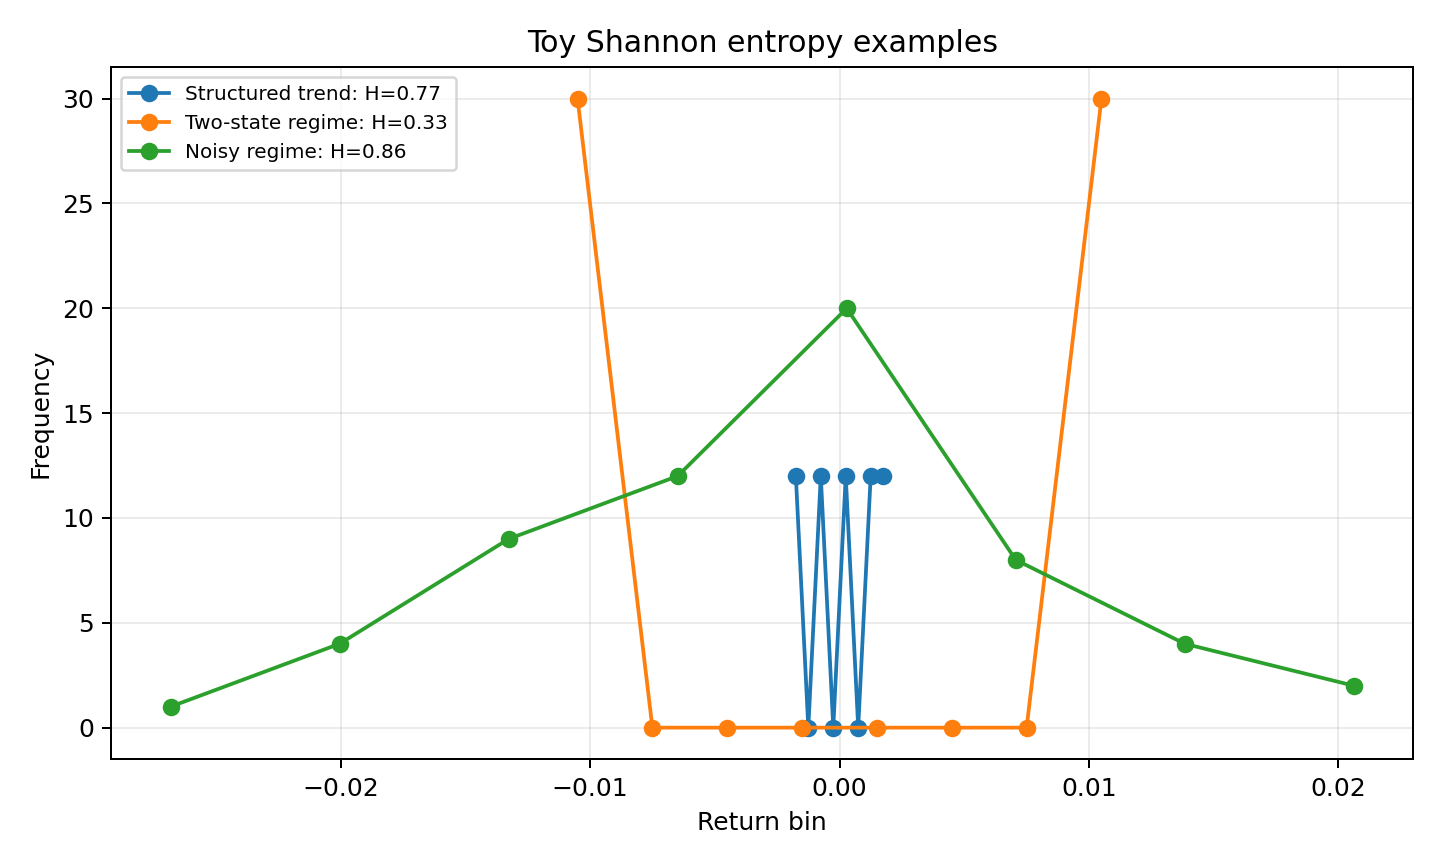
\includegraphics[width=0.82\linewidth]{toy_entropy_example.png}
\caption{Toy example showing how normalized Shannon entropy changes with return concentration.}
\end{figure}

The important point is that entropy is not a return forecast: it is a measure of order versus disorder. In this project it is used \emph{only} to classify the regime; the expected-return input is the plain rolling mean, which entropy does not scale.

\subsection{From entropy to weights: a full mini-allocation}
\label{sec:toy-allocation}

The example above isolates the entropy step. To show the \emph{whole} algorithm solving the \emph{portfolio} problem on a reduced scale, take a four-name universe $\{A,B,C,D\}$ with a short history of eight daily returns per name (in \%); Figure~\ref{fig:toy-allocation} summarizes the inputs and the resulting weights.

\begin{center}
\small
\begin{tabular}{lrrrrrrrr}
\toprule
Stock & \multicolumn{8}{c}{Daily returns (\%)}\\
\midrule
$A$ & $0.6$ & $0.8$ & $0.5$ & $0.7$ & $0.9$ & $0.6$ & $0.8$ & $0.7$\\
$B$ & $2.0$ & $-1.8$ & $1.5$ & $-2.2$ & $0.3$ & $1.9$ & $-1.0$ & $0.8$\\
$C$ & $1.2$ & $-0.3$ & $0.9$ & $1.5$ & $-0.6$ & $1.1$ & $0.4$ & $0.8$\\
$D$ & $-0.2$ & $-0.5$ & $0.1$ & $-0.4$ & $-0.3$ & $0.0$ & $-0.6$ & $0.2$\\
\bottomrule
\end{tabular}
\end{center}

\paragraph{Step 1 --- entropy and the rolling-mean expected return.} Running \textsc{ShannonEntropy} ($B=8$) on each window gives the per-name entropy $H_i$ (used only to set the regime); the expected-return input is the plain rolling mean $\widehat\mu_i=\bar r_i$, which entropy does not scale:

\begin{center}
\small
\begin{tabular}{lrr}
\toprule
Stock & $H_i$ & $\widehat\mu_i=\bar r_i$\\
\midrule
$A$ & $0.750$ & $0.700\%$\\
$B$ & $0.719$ & $0.187\%$\\
$C$ & $0.833$ & $0.625\%$\\
$D$ & $0.917$ & $-0.213\%$\\
\bottomrule
\end{tabular}
\end{center}

\paragraph{Step 2 --- regime and cap.} The universe-average entropy is $\bar H=\tfrac14(0.750+0.719+0.833+0.917)=0.805$. In a full run this is compared with its rolling $33/67$ bands; for the toy we place it in the \textbf{Bullish} regime, which sets the per-name cap to $c=30\%$ (minimum $0$). The cap policy is a single lookup: $c\gets$ \texttt{REGIME\_TO\_MAX\_WEIGHT[phase]}.

\paragraph{Step 3 --- covariance.} The trailing sample covariance of the four windows is (entries $\times 10^4$)
\[
\Sigma\times10^4=
\begin{pmatrix}
\phantom{-}0.017 & -0.130 & -0.074 & -0.024\\
-0.130 & \phantom{-}2.770 & \phantom{-}0.315 & \phantom{-}0.360\\
-0.074 & \phantom{-}0.315 & \phantom{-}0.548 & \phantom{-}0.080\\
-0.024 & \phantom{-}0.360 & \phantom{-}0.080 & \phantom{-}0.084
\end{pmatrix}.
\]
Note that $A$ has by far the smallest variance and is \emph{negatively} correlated with $B$.

\paragraph{Step 4 --- the SLSQP solve.} With risk aversion $\lambda=4$, \textsc{Slsqp} minimizes $\tfrac{\lambda}{2}w^\top\Sigma w-\widehat\mu^\top w$ subject to $\sum_i w_i=1$ and $0\le w_i\le 0.30$. The solution is
\[
w_A=30.0\%,\qquad w_B=30.0\%,\qquad w_C=30.0\%,\qquad w_D=10.0\%.
\]
The three names with the best risk-adjusted appeal --- $A$ (by far the lowest variance), $C$ (highest $\widehat\mu$), and $B$ (a non-trivial mean and, crucially, a \emph{diversifying} negative correlation with $A$) --- are all pushed to the $30\%$ cap. $D$ absorbs the remaining $10\%$: with three caps binding at $30\%$, the budget $\sum_i w_i=1$ must place the last $10\%$ somewhere, and $D$'s very low variance makes it the least costly filler despite its slightly negative $\widehat\mu$.

\paragraph{The other regime, for contrast.} Had the same day been classified \textbf{Bearish}, the optimizer would be skipped and the book set directly to equal weight, $w_A=w_B=w_C=w_D=25\%$ (the $1/n$ posture; equivalently the relaxed $10\%$ cap with $n=4$). The same machinery therefore speculates (concentrates at the $30\%$ cap) in the ordered regime and diversifies (equal weight) in the disordered one --- the whole strategy, on four stocks.

\begin{figure}[H]
\centering
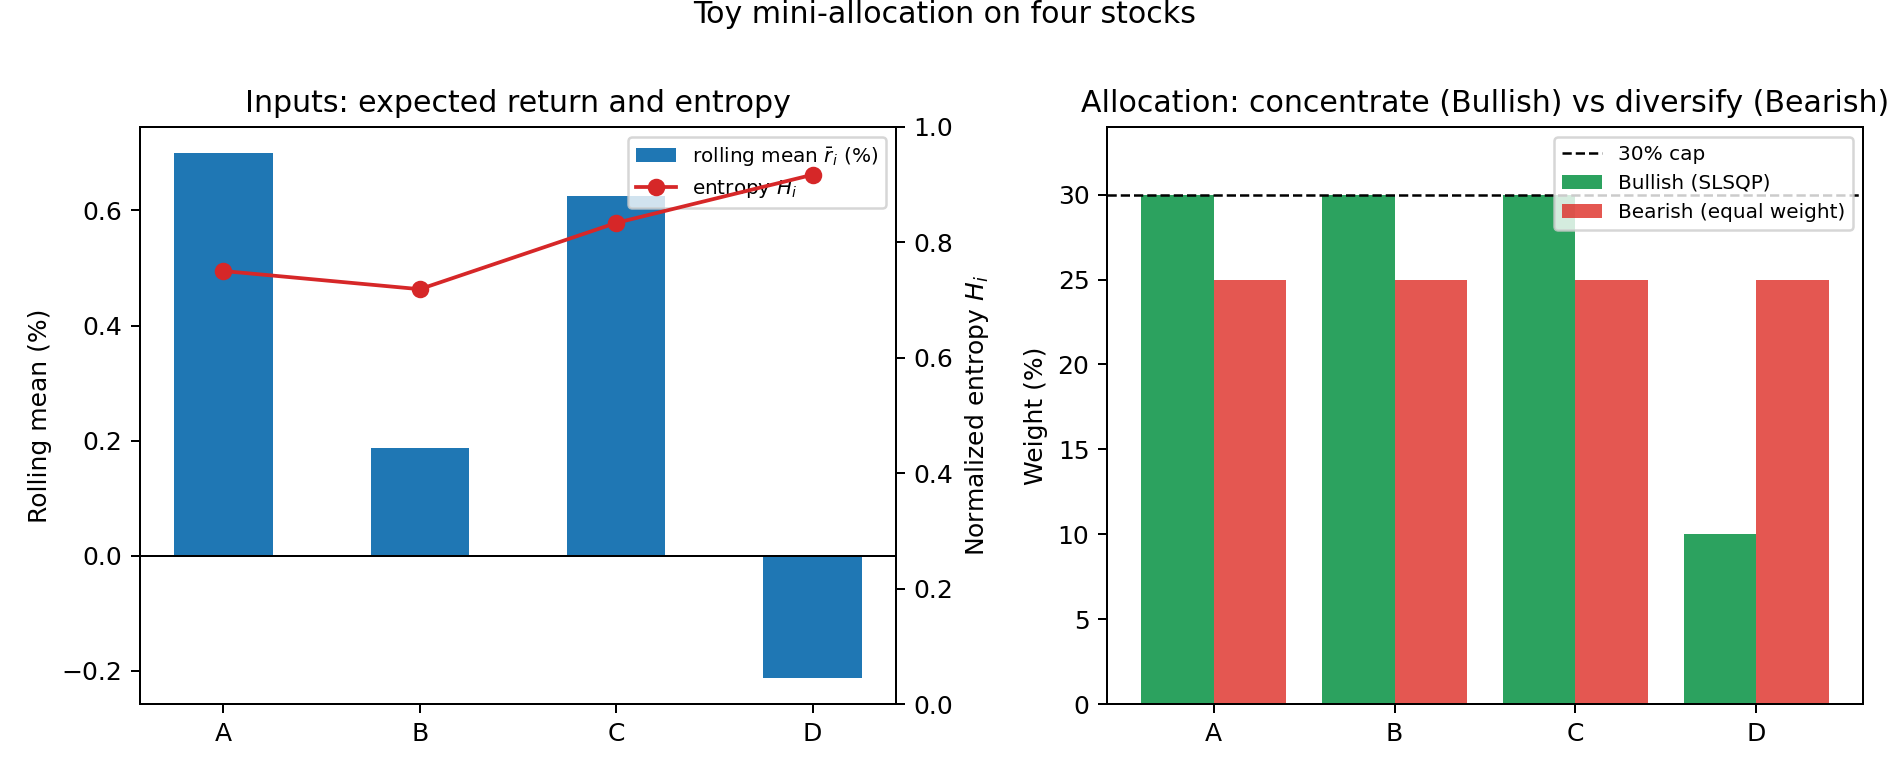
\includegraphics[width=0.96\linewidth]{toy_allocation.png}
\caption{The toy mini-allocation, produced by the same code as the real backtest. \textbf{Left:} the per-name inputs --- the rolling mean $\bar r_i$ (blue bars, left axis) and the entropy $H_i$ (red, right axis). \textbf{Right:} the resulting weights --- the Bullish SLSQP book pushes the three best risk-adjusted names ($A$, $B$, $C$) to the $30\%$ cap and uses the low-variance $D$ as filler, while the Bearish gear would simply hold the $25\%$ equal-weight book. Entropy sets only \emph{which} gear is engaged, never the weights inside it.}
\label{fig:toy-allocation}
\end{figure}

\section{Computational Complexity Analysis}
\label{sec:complexity}

\subsection{Overview}

The portfolio optimization pipeline integrates several algorithms with distinct computational profiles. This section documents the time and space complexity of each stage and justifies the choice of algorithms and data structures.

The real problem solved by the pipeline is operational --- build a feasible long-only portfolio every trading day over the dynamic top-10 of the S\&P 500 --- but its algorithmic substance lies almost entirely in one stage. The \emph{rolling-entropy computation is the core contribution of this project}: it is the window-adaptive histogram method analyzed below, and, as the propositions below establish, it is the single term that dominates the end-to-end cost and sets an asymptotic floor. The allocation that consumes the entropy signal is deliberately trivial by comparison: the per-name cap is read straight off the regime ($30\%$ Bullish, $15\%$ Neutral) and a standard SLSQP mean-variance solver enforces it, with no calibration and no candidate grid; in the Bearish regime the solver is skipped entirely and the book is equal weight. Accordingly, this section treats the entropy computation as the algorithmic heart and the optimizer as a small bounded-size subproblem.

\subsection{Shannon Entropy Computation}

\begin{definition}[Complexity of normalized Shannon entropy]
The rolling Shannon entropy for asset $i$ over a window of $n$ observations and $B$ histogram bins is computed as:
\[
H_i = -\frac{1}{\log_2 B} \sum_{b=1}^{B} p_b \log_2(p_b)
\]
where $p_b$ is the empirical probability of bin $b$.
\end{definition}

\begin{proposition}[Complexity of shannon\_entropy function]
On one window of $W$ returns with $B$ fixed bins, the routine runs in five steps:
\begin{enumerate}[label=(\roman*)]
    \item \textbf{Input cleaning} --- drop non-finite values in one pass: $O(W)$.
    \item \textbf{Histogram construction} (\texttt{np.histogram}) --- scan the window for $[\min,\max]$ to place the equal-width edges ($O(W)$), then assign all $W$ points to bins ($O(W)$): $O(W)$.
    \item \textbf{Count $\to$ probability normalization} ($p_b=c_b/W$): $O(B)$.
    \item \textbf{Shannon sum} ($-\sum_b p_b\log_2 p_b$ over non-empty bins): $O(B)$.
    \item \textbf{Final normalization} (divide by $\log_2 B$): $O(1)$.
\end{enumerate}
Summing the steps gives \textbf{time} $\Theta(W+B)=\Theta(W)$ for fixed, small $B$ (here $W=126\gg B=8$). \textbf{Best and worst case coincide at $\Theta(W)$}: whatever the data, the histogram must inspect every value of the window both to find the range and to bin it, so no input makes the routine sub-linear in $W$, and none makes it super-linear. \textbf{Space} is $O(B)$ for the bin counts, plus a transient $O(W)$ window copy. The \texttt{numpy.ndarray} window enables a single C-level histogram pass with no Python-loop overhead.
\end{proposition}

\subsection{Rolling Entropy Signal}

Here $N$ is the number of ticker columns in the price panel --- \emph{every} name that is ever in the top-10 over the sample ($N\approx 33$--$90$), not the $K=10$ active on a given day --- because the rolling entropy is computed on all columns before the active mask is applied.

\begin{proposition}[Complexity of rolling entropy computation]
Sliding the $W=126$ window over $T$ trading days and $N$ columns:
\begin{enumerate}[label=(\roman*)]
    \item \textbf{Time Complexity:} $\Theta(T \times N \times W)$.
    \begin{itemize}
        \item There are $O(T)$ windows per column and $N$ columns, each window $O(W)$ (Proposition above).
        \item The companion rolling \texttt{mean}/\texttt{std} are $O(TN)$ each (incremental moments) and are dominated.
        \item The long-format \texttt{stack}/\texttt{merge}/\texttt{sort} is $O(TN\log(TN))$, also dominated since $W=126>\log_2(TN)$.
    \end{itemize}
    \item \textbf{Space Complexity:} $O(T \times N)$ for the panel and for each of the rolling output matrices (entropy, mean, volatility).
    \item \textbf{Data Structure Justification:} \texttt{pandas.rolling().apply(raw=True)} hands each window to the histogram kernel as a contiguous NumPy array; the only ``algorithmic'' structure is the implicit equal-width histogram whose edges are recomputed from each window's $[\min,\max]$.
\end{enumerate}
\end{proposition}

\begin{remark}[Would monotone deques give $O(1)$ rolling entropy? Why a faster $\min/\max$ does not help]
\label{rem:deque}
A natural idea is to keep the window's $\min$ and $\max$ with two \emph{monotone deques}, which maintain a sliding minimum/maximum in $O(1)$ amortized per step. This does work --- but it solves only the \emph{range} of the window, not the entropy.

The factor $W$ cannot be removed while the bin edges are \emph{window-adaptive}. Because \texttt{np.histogram} derives the edges from each window's own $[\min,\max]$, when the range changes the bin \emph{boundaries} move; values already inside the window can then fall into different bins, so the previously accumulated counts become invalid and the $B$ counts must be rebuilt by a full $O(W)$ pass. Thus monotone deques plus a dynamically re-binned histogram still cost $\Theta(W)$ per window and $\Theta(TNW)$ in total: the deque removes only a constant factor.

To genuinely update in $O(1)$ with respect to $W$ one must \emph{fix} the bin edges in advance. A concrete online scheme: choose regular bins on $[-5\%,+5\%]$ with one tail bin for $x<-5\%$ and one for $x>+5\%$; keep a \emph{circular buffer} of the last $W$ returns, a parallel buffer of \emph{the bin index} each stored return was assigned to, and an array of bin \emph{counts}. On each new day, decrement the count of the bin of the return leaving the window and increment the count of the bin of the entering return ($O(1)$ amortized, plus $O(B)$ to recompute $H$ from the counts). This makes rolling entropy $O(TN)$ overall and is causal. We do \emph{not} adopt it here: fixed edges redefine the feature --- entropy would then depend on the absolute return scale rather than on the window's shape, re-coupling it to volatility as quantified in Section~\ref{sec:binning} --- and would change every downstream number. Efficiency and the choice of binning are therefore the same design decision; the current version keeps window-adaptive bins and stays $\Theta(W)$ per window.
\end{remark}

\subsection{Mean-Variance Optimization}

\begin{proposition}[Complexity of SLSQP optimizer]
The daily loop runs over $T$ dates with $K\le 10$ active assets and $I$ iterations per solve. The simplified project has \emph{no} candidate grid: the per-name cap is read directly from the regime, so the grid factor of the original project is gone.
\begin{enumerate}[label=(\roman*)]
    \item \textbf{Time Complexity:} $O\!\big(T \times (W K^2 + I K^3)\big)$.
    \begin{itemize}
        \item Each day rebuilds the trailing $K\times K$ covariance from $W$ rows: $O(W K^2)$.
        \item Each SLSQP iteration solves a small dense KKT system: $O(K^3)$, with $I\approx 5$--$10$. The solver is called only in the Bullish/Neutral regimes; Bearish days skip it (equal weight), so the $O(IK^3)$ term is incurred on a strict subset of days.
        \item With $K\le 10$ both terms are tiny constants per day, so the loop is effectively $O(T)$.
    \end{itemize}
    \item \textbf{Space Complexity:} $O(K^2)$ per day for the covariance and constraint matrices.
    \item \textbf{Algorithm Justification:}
    \begin{itemize}
        \item SLSQP chosen over interior-point for stability on small $K$ with simple linear constraints.
        \item Analytic gradient $\lambda\Sigma_t w-\widehat\mu_t$ avoids finite differences.
        \item Regime-conditional action: Bullish/Neutral set $c_t\in\{0.30,0.15\}$ and call SLSQP; Bearish skips the solver and uses equal weight --- no walk-forward search.
    \end{itemize}
\end{enumerate}
\end{proposition}

\subsection{Allocation cost ladder: from $O(N)$ to $O(N^3)$}
\label{sec:naive}

How much computation does the allocation rule itself deserve? It is instructive to place three allocation rules on a \emph{cost ladder} for a single day with $N$ active names, and to ask what the extra cost buys (the empirical comparison is in Section~\ref{sec:simulations}).

\begin{enumerate}[label=\arabic*.]
    \item \textbf{Equal weight} --- $w_i=1/N$. No estimation at all: \textbf{best and worst case $\Theta(N)$} just to write the vector. This is also the Bearish gear of our strategy.
    \item \textbf{Naive max-Sharpe} --- a sensible first idea is to pick the names with the best risk-adjusted history: compute each name's rolling Sharpe $\widehat s_i=\bar r_i/\sigma_i$ from quantities already available, and set $w_i\propto\max(\widehat s_i,0)$ (equal weight if none is positive). Computing the scores and normalizing is $\Theta(N)$; the weights are then saved and applied. \textbf{Best case $\Theta(N)$} (no sorting needed for the proportional rule); if instead one selected and ranked a top-$k$ subset, a full sort makes it $\Theta(N\log N)$ \textbf{worst case}. Either way it is essentially free and uses \emph{no} optimizer.
    \item \textbf{Regime-adaptive mean-variance (SLSQP)} --- the strategy of this report. Beyond the $\Theta(W N)$ to rebuild the trailing covariance, each solve performs $I$ iterations whose dominant step is a dense linear system in $N$ variables, $\Theta(N^3)$ per iteration. \textbf{Best case} (immediate convergence, $I=O(1)$) is $\Theta(WN^2+N^3)$ per day; \textbf{worst case} is $\Theta(WN^2+I_{\max}N^3)$ with $I_{\max}$ the iteration cap. The $N^3$ term is what makes a true optimizer qualitatively more expensive than the two cheaper rules.
\end{enumerate}

The ladder makes the trade-off explicit: equal weight is $\Theta(N)$ and ignores the data, the naive max-Sharpe rule is $\Theta(N)$--$\Theta(N\log N)$ and uses first moments only, and the mean-variance solve is $\Theta(N^3)$ but actually uses the covariance structure (so it can exploit diversifying negative correlations, as in the toy example). Whether the $N^3$ cost is worth paying is an empirical question, answered for our sample in Section~\ref{sec:simulations}; with $N\le 10$ the absolute cost is small, but the asymptotic gap is the right lens for larger universes.

\subsection{Data Preparation, Market Phases, and Statistics}

\begin{proposition}[Complexity of the remaining stages]
\begin{enumerate}[label=(\roman*)]
    \item \textbf{Active-universe construction:} $O(T N)$. It fills a dense $T\times N$ boolean membership frame (month-end top-10 forward-filled to daily dates); this is the dominant cost of data preparation. It is built by a vectorized membership lookup --- a cached map from each distinct monthly top-10 set to its column mask --- so the inner $O(K)$ work runs once per unique set rather than once per day, avoiding a per-date label scatter.
    \item \textbf{Market phases:} the regime statistics act on a \emph{single} proxy series, so the rolling product/quantile/std are $O(T W)$ on one series (cheap) and the daily Bullish/Neutral/Bearish label is $O(T)$.
    \item \textbf{Performance metrics:} $O(T)$ single-pass per strategy (cumulative product for final wealth, running-max scan for drawdown, mean/variance for Sharpe), hence $O(ST)$ over $S=4$ strategies; crisis windows add $O(CT)$ with $C\approx 4$.
    \item \textbf{Space Complexity:} $O(T)$ per return series; $O(TN)$ for the active-universe frame.
\end{enumerate}
\end{proposition}

\subsection{End-to-End Pipeline}

\begin{proposition}[Total pipeline complexity]
The complete pipeline from raw returns to final metrics:
\begin{enumerate}[label=(\roman*)]
    \item \textbf{Dominant term:} $\Theta(T \times N \times W)$ from the rolling entropy signal. Everything else is lower order: $O(TN)$ data preparation, $O\!\big(T(WK^2+IK^3)\big)$ MVO with $K\le 10$, and $O(T)$ statistics.
    \item \textbf{Memory footprint:} $O(T \times N)$ for the price panel and the entropy/weight matrices.
    \item \textbf{Practical runtime:} of the order of a minute for the full run ($T\approx 6300$, $N\approx 33$--$90$); the rolling entropy and the daily SLSQP loop are the largest compute terms (a few tens of seconds together), and rendering the report figures is a comparable fixed cost.
\end{enumerate}
\end{proposition}

\begin{remark}[Constant-factor speedups that preserve every number]
Three changes cut wall-clock without altering any output (verified bit-for-bit on all exported tables): the active-universe fill is vectorized as above; the daily optimizer detects its active set with positional NumPy masks instead of per-ticker label lookups; and the degenerate-window guard in \texttt{shannon\_entropy} is dropped because the histogram already maps a constant window to a single bucket ($H=0$). None of these lowers the asymptotic class --- they remove interpreted-Python and pandas-label-lookup constants, which is where the measured time actually went.
\end{remark}

\section{Algorithm Analysis}

\subsection{Data structures used}

The implementation uses simple data structures on purpose:
\begin{enumerate}[label=\arabic*.]
    \item \textbf{Price and return matrices}: dense \texttt{pandas.DataFrame} objects indexed by date and ticker.
    \item \textbf{Active-universe matrix}: a boolean date-by-ticker matrix where one means the ticker belongs to the current top-10 set.
    \item \textbf{Rolling matrices}: rolling entropy, rolling mean (the prediction $\widehat\mu=\bar r$), and rolling volatility are stored as aligned date-by-ticker matrices for numerical operations.
    \item \textbf{Long diagnostic tables}: active ticker-date observations are stacked into long tables for the per-name weight and overweight/underweight tilt diagnostics and figures.
    \item \textbf{Portfolio diagnostic table}: each trading date stores active count, invested count, bound counts, solver success, and feasibility residuals.
\end{enumerate}

\subsection{Computational complexity}

The asymptotic costs were derived in detail in the Computational Complexity Analysis section: with $T$ trading dates, $N$ distinct top-10 tickers over the sample, window $W$, $B$ bins, and $K\le 10$ active names, the rolling entropy dominates at $\Theta(TNW)$ --- a \emph{floor}, because the histogram edges are window-adaptive --- while the daily optimizer is a small dense problem in $K$ variables and is therefore effectively linear in $T$. Rather than repeat that derivation, this section concentrates on the data structures that realize those costs and on why the implementation is acceptable in practice.

The allocation layer reads its action directly from the current entropy regime: a per-name cap $c_t\in\{0.30,0.15\}$ (zero minimum) with an SLSQP solve in Bullish/Neutral, and an explicit equal-weight book in Bearish. There is no candidate grid, no expanding-bound search, and nothing to recalibrate. Each SLSQP solve is independent and starts from the equal-weight vector (always feasible because $c_t\ge 1/n$); the routine is called on Bullish/Neutral days only. This keeps the algorithm auditable and avoids any repeated rescanning of the historical return table, because the action is set by the regime rather than chosen by evaluating candidates on past data.

\subsection{Why this implementation is acceptable}

The implementation favors transparent data structures over hidden state. Adjusted prices, simple returns, active universe, entropy, rolling-mean expected returns, the per-name regime cap, weights, and feasibility residuals are all exported as CSV files. The optimizer also records whether SLSQP succeeded, so the report can verify that the numerical solution satisfies the constraints.

\section{Simulations}
\label{sec:simulations}

\subsection{Experimental setup}

The simulation uses daily price-index inputs from 2001-01-31 through 2025-12-31. The portfolio evaluation begins on 2002-01-31, once the 126-trading-day rolling history and the rolling 504-day entropy-quantile bands have both warmed up, giving 6{,}015 optimized trading days. The monthly top-10 universe always contains 10 names and contains 33 distinct tickers over the full sample. Every figure and table in this report is produced by a single, self-contained notebook that runs unchanged in Google Colab; the three input CSVs are read from one editable \texttt{DATA\_DIR} path variable, so moving the data to another file system is a one-line change.

The main parameters are:
\begin{enumerate}[label=\arabic*.]
    \item entropy lookback: $W=126$ trading days;
    \item entropy bins: $B=8$;
    \item active universe size: $K=10$;
    \item per-name cap from the regime: 30/15/10\% (Bullish/Neutral/Bearish);
    \item minimum per-name weight: 0 (always);
    \item regime quantile window: $W_H=504$ trading days with 33rd/67th percentile bands;
    \item risk aversion: $\lambda=4$;
    \item optimizer: SLSQP in the Bullish/Neutral regimes; equal weight in Bearish;
    \item benchmarks: a naive max-Sharpe top-10, the dynamic equal-weight top-10, and the S\&P 500 total-return buy-and-hold (no rebalancing).
\end{enumerate}

% (company-paths section removed in the simplified project)

\subsection{Entropy signal through time}

\begin{figure}[H]
\centering
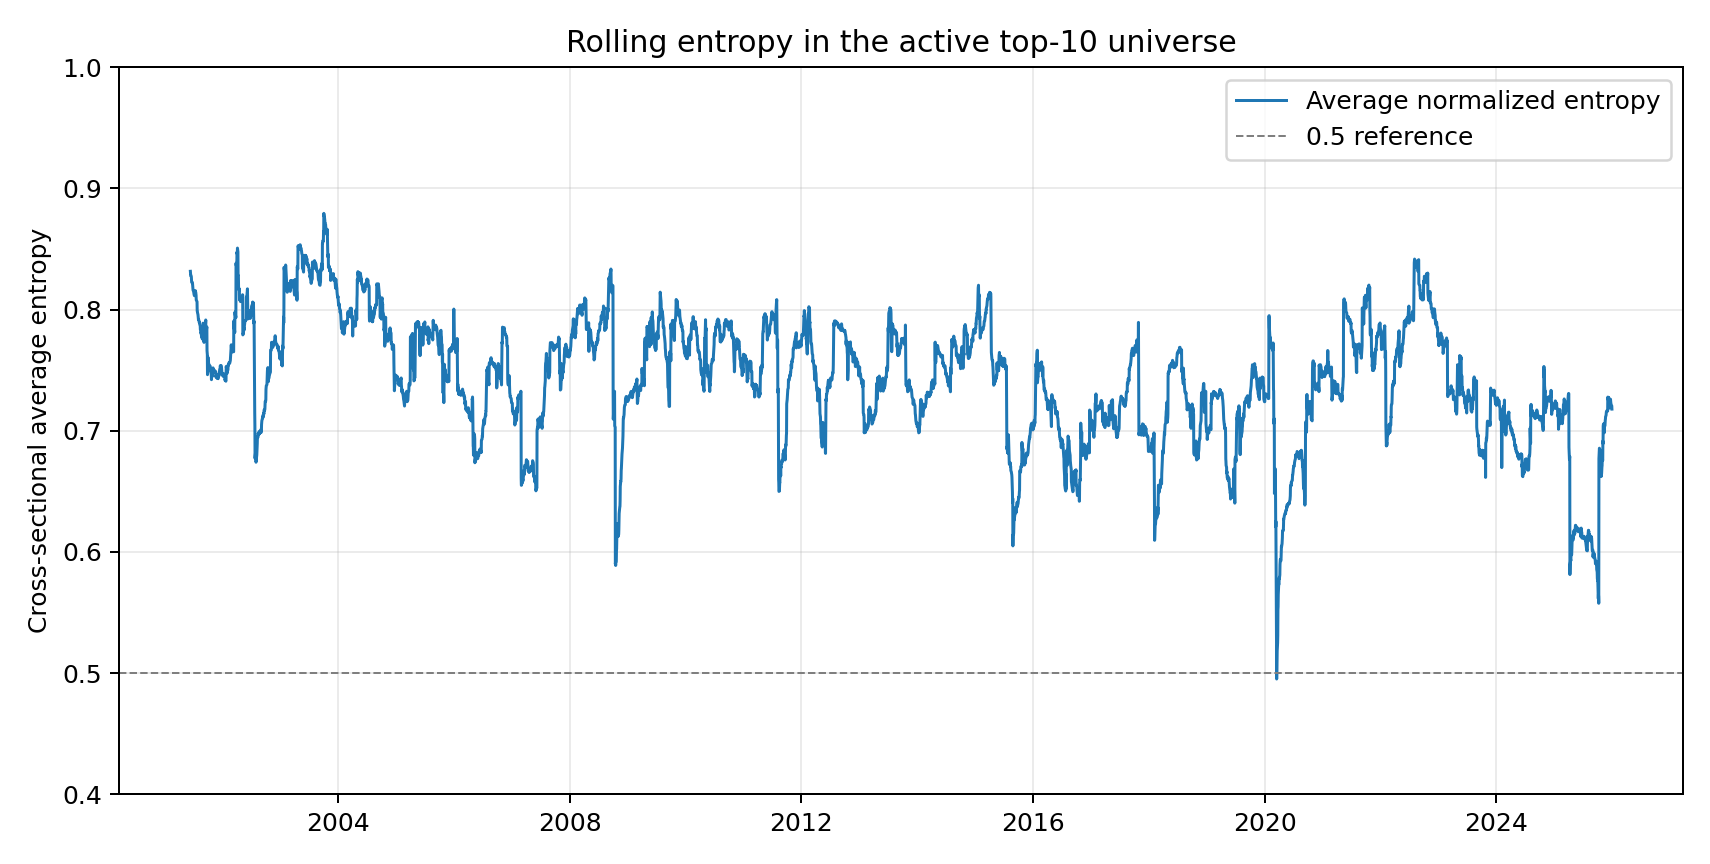
\includegraphics[width=0.86\linewidth]{entropy_overview.png}
\caption{Average normalized entropy in the active top-10 universe. Low entropy marks an ordered market in which the strategy concentrates; high entropy marks a disordered market in which it diversifies toward equal weight.}
\end{figure}

Entropy is exactly the dial the strategy watches: it tells ordered markets from disordered ones so the allocation knows which gear to engage. When the average entropy line rises, recent return distributions are more spread across states --- a disordered market in which the strategy diversifies toward equal weight. When it falls, recent returns are more concentrated --- an ordered market in which the strategy concentrates. Entropy enters \emph{only} this regime decision; it does not modify the return prediction.

\begin{figure}[H]
\centering
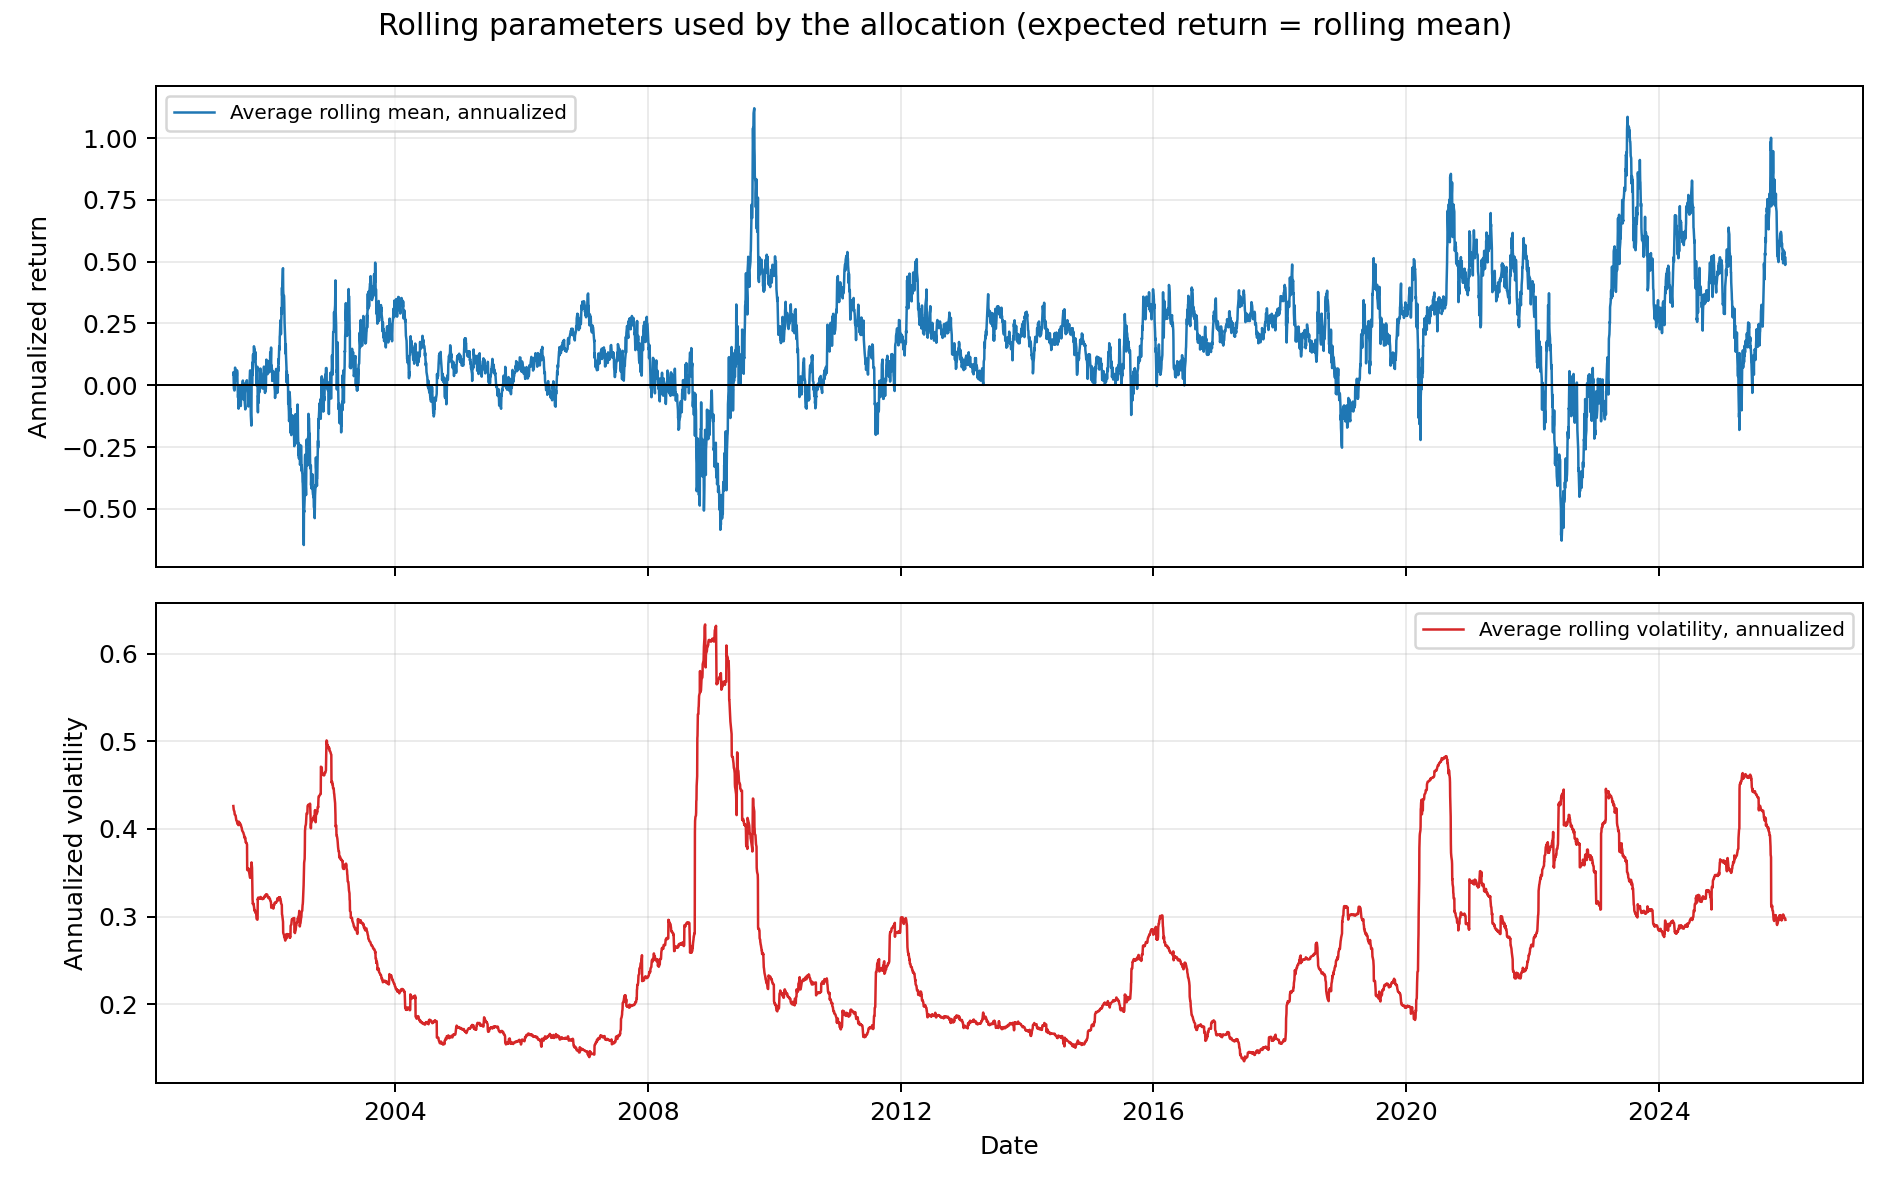
\includegraphics[width=0.96\linewidth]{rolling_signal_parameters.png}
\caption{Rolling parameters that feed the allocation: the annualized rolling mean --- the expected-return input $\widehat\mu=\bar r$ (top) --- and the annualized rolling volatility (bottom). The average entropy is shown separately in the figure above.}
\end{figure}

\subsection{Portfolio performance}

The strategy is compared with three no-look-ahead benchmarks: the naive max-Sharpe top-10 of Section~\ref{sec:naive}, the dynamic equal-weight top-10, and the S\&P 500 total-return index held without rebalancing (buy-and-hold). All series are rebased to 1 at the first optimized day.

\begin{figure}[H]
\centering
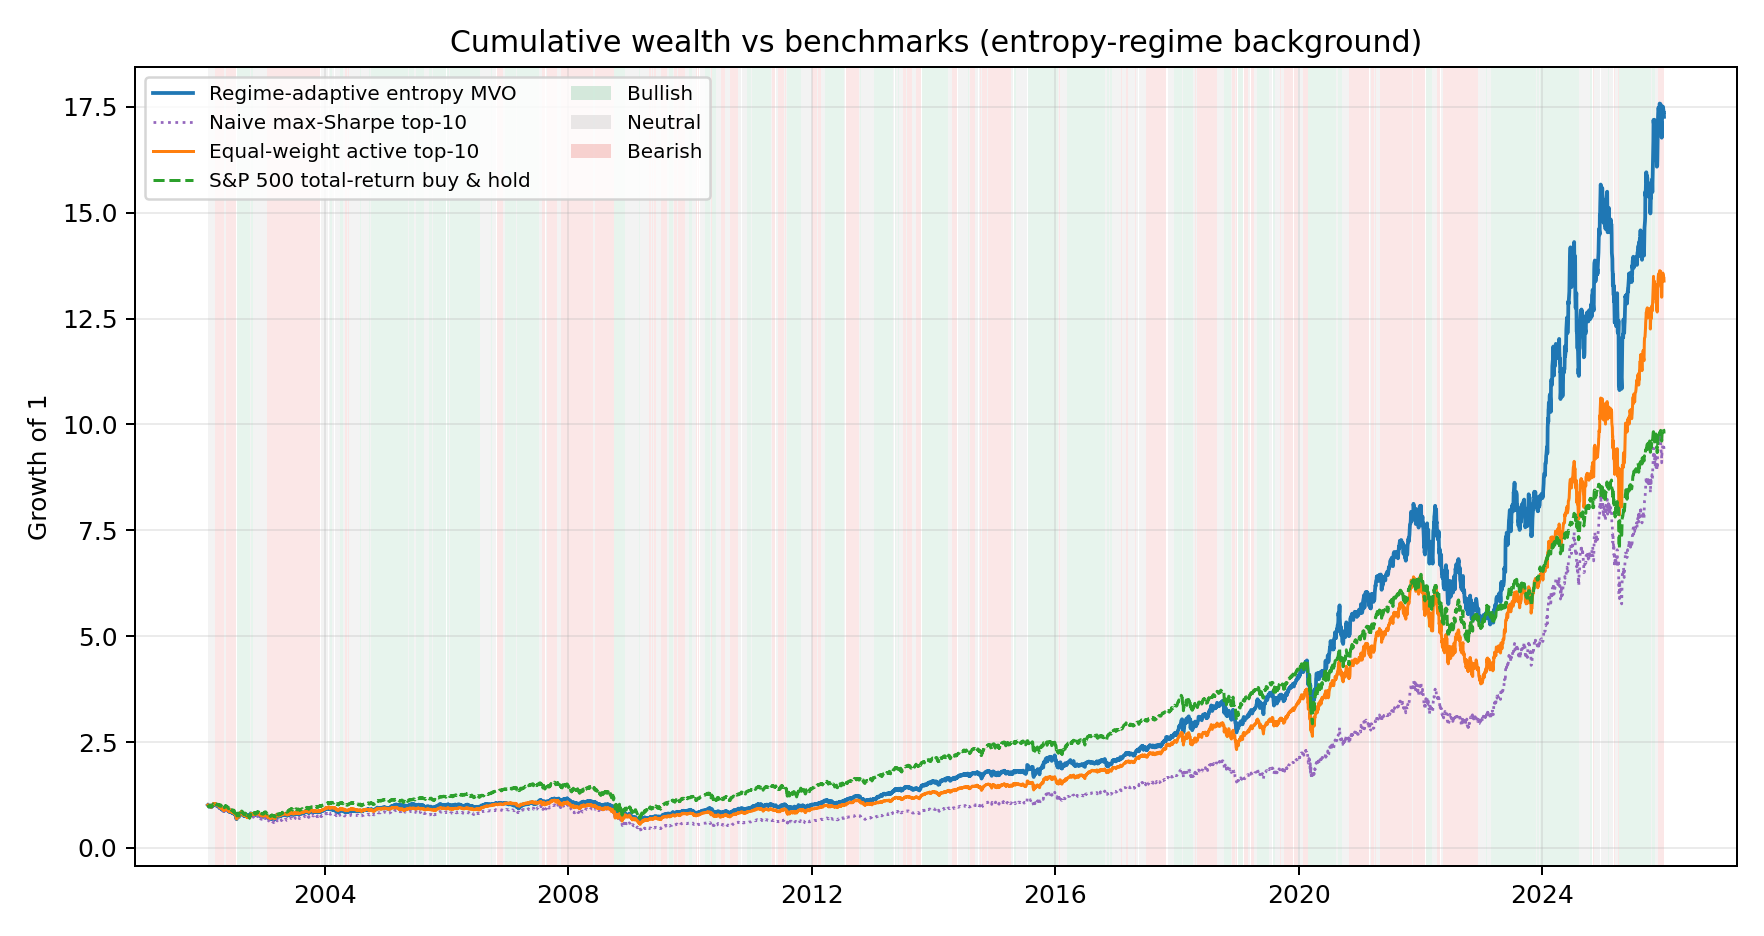
\includegraphics[width=0.86\linewidth]{cumulative_returns.png}
\caption{Cumulative wealth of the entropy-regime allocation versus the naive max-Sharpe top-10, the equal-weight top-10, and the S\&P 500 total-return buy-and-hold. Background colors identify the estimated Bullish, Neutral, or Bearish phase --- the strategy's three gears: concentrate (Bullish, ordered), balanced (Neutral), and equal-weight/diversify (Bearish, disordered).}
\end{figure}

\begin{table}[H]
\centering
\begingroup
\footnotesize
\setlength{\tabcolsep}{3.5pt}
\resizebox{0.92\linewidth}{!}{\begin{tabular}{lrrrrr}
\hline
Strategy & Ann. return & Ann. vol & Sharpe & Max DD & Final wealth \\
\hline
Regime-adaptive entropy MVO & 12.68\% & 21.09\% & 0.601 & -47.42\% & 17.265 \\
Naive max-Sharpe top-10 & 9.85\% & 21.01\% & 0.469 & -58.85\% & 9.414 \\
Equal-weight active top-10 & 11.48\% & 20.84\% & 0.551 & -50.36\% & 13.387 \\
S\&P 500 total-return buy \& hold & 10.03\% & 19.16\% & 0.523 & -54.80\% & 9.787 \\
\hline
\end{tabular}
}
\endgroup
\caption{Performance metrics for the regime-adaptive entropy strategy, the naive max-Sharpe top-10, the equal-weight top-10, and the S\&P 500 total-return buy-and-hold benchmark, over 2002--2025 (6{,}015 optimized days).}
\end{table}

Over the full sample the regime-adaptive strategy is the strongest on every reported metric: a final wealth of $17.3\times$ against $13.4\times$ for the equal-weight top-10, $9.8\times$ for the S\&P 500, and $9.4\times$ for the naive max-Sharpe rule; an annualized return of $12.7\%$ versus $11.5\%$, $10.0\%$, and $9.8\%$; the highest Sharpe ratio ($0.60$ against $0.55$, $0.52$, and $0.47$); and the shallowest maximum drawdown ($-47.4\%$ against $-50.4\%$, $-54.8\%$, and $-58.9\%$).

This is the empirical answer to the cost-ladder question of Section~\ref{sec:naive}. The cheapest non-trivial rule --- naive max-Sharpe, $\Theta(N)$ --- is in fact the \emph{worst} performer here: chasing names by past Sharpe alone concentrates into recent winners and suffers the deepest drawdown, because it ignores the covariance structure. Equal weight ($\Theta(N)$) is a solid, hard-to-beat baseline. The $\Theta(N^3)$ mean-variance solve, gated by the entropy regime, is what actually adds value: it exploits diversifying correlations in the ordered regimes and steps aside into equal weight in the disordered ones. The extra computational cost buys a genuine improvement here, though one should remember that with $N\le 10$ the absolute cost is negligible; for much larger universes the $N^3$ term would have to be weighed against the gain.

\subsection{Behavior during crisis windows}

The crisis check isolates four stressed subperiods: the global financial crisis, the 2011 Euro debt and U.S. downgrade episode, the COVID crash, and the 2022 inflation-and-rates bear market. These are precisely the disordered, high-entropy stretches in which the strategy should shift into its diversifying gear and pull every name toward the equal-weight Bearish cap. Each panel in Figure \ref{fig:crisis-behavior} rebases wealth to 1 at the start of the crisis window, so the comparison is local to that episode rather than dominated by the full-sample compounding path.

\begin{figure}[H]
\centering
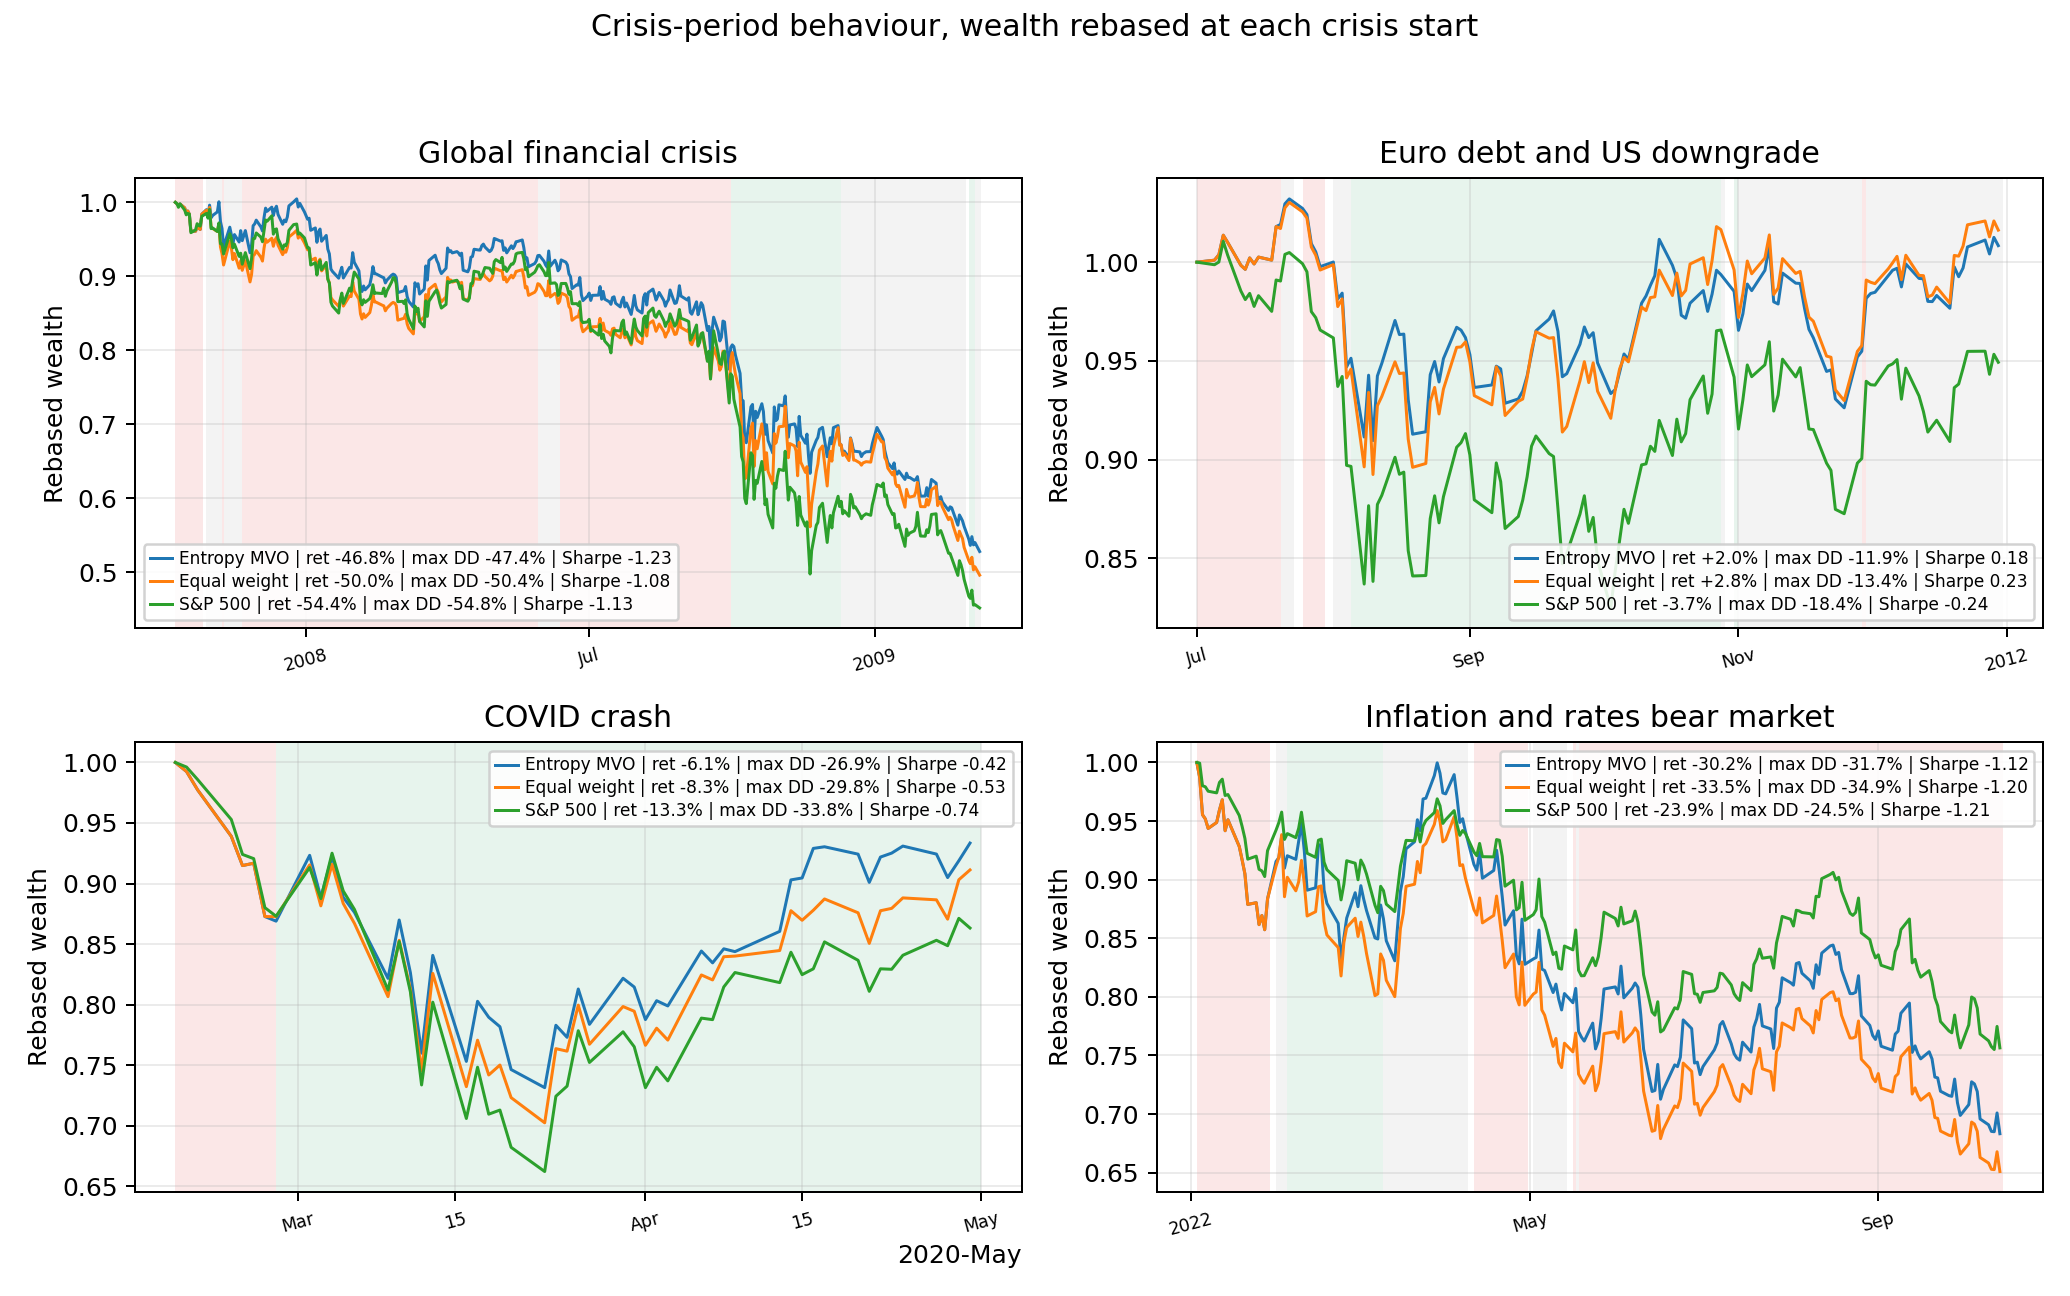
\includegraphics[width=0.96\linewidth]{crisis_behavior.png}
\caption{Crisis-period behavior of the entropy-regime mean-variance portfolio versus the dynamic equal-weight benchmark. These disordered episodes are where the strategy engages its diversifying gear, so its path tracks the equal-weight benchmark closely. Wealth is rebased to 1 at the start of each crisis window.}
\label{fig:crisis-behavior}
\end{figure}

\begin{figure}[H]
\centering
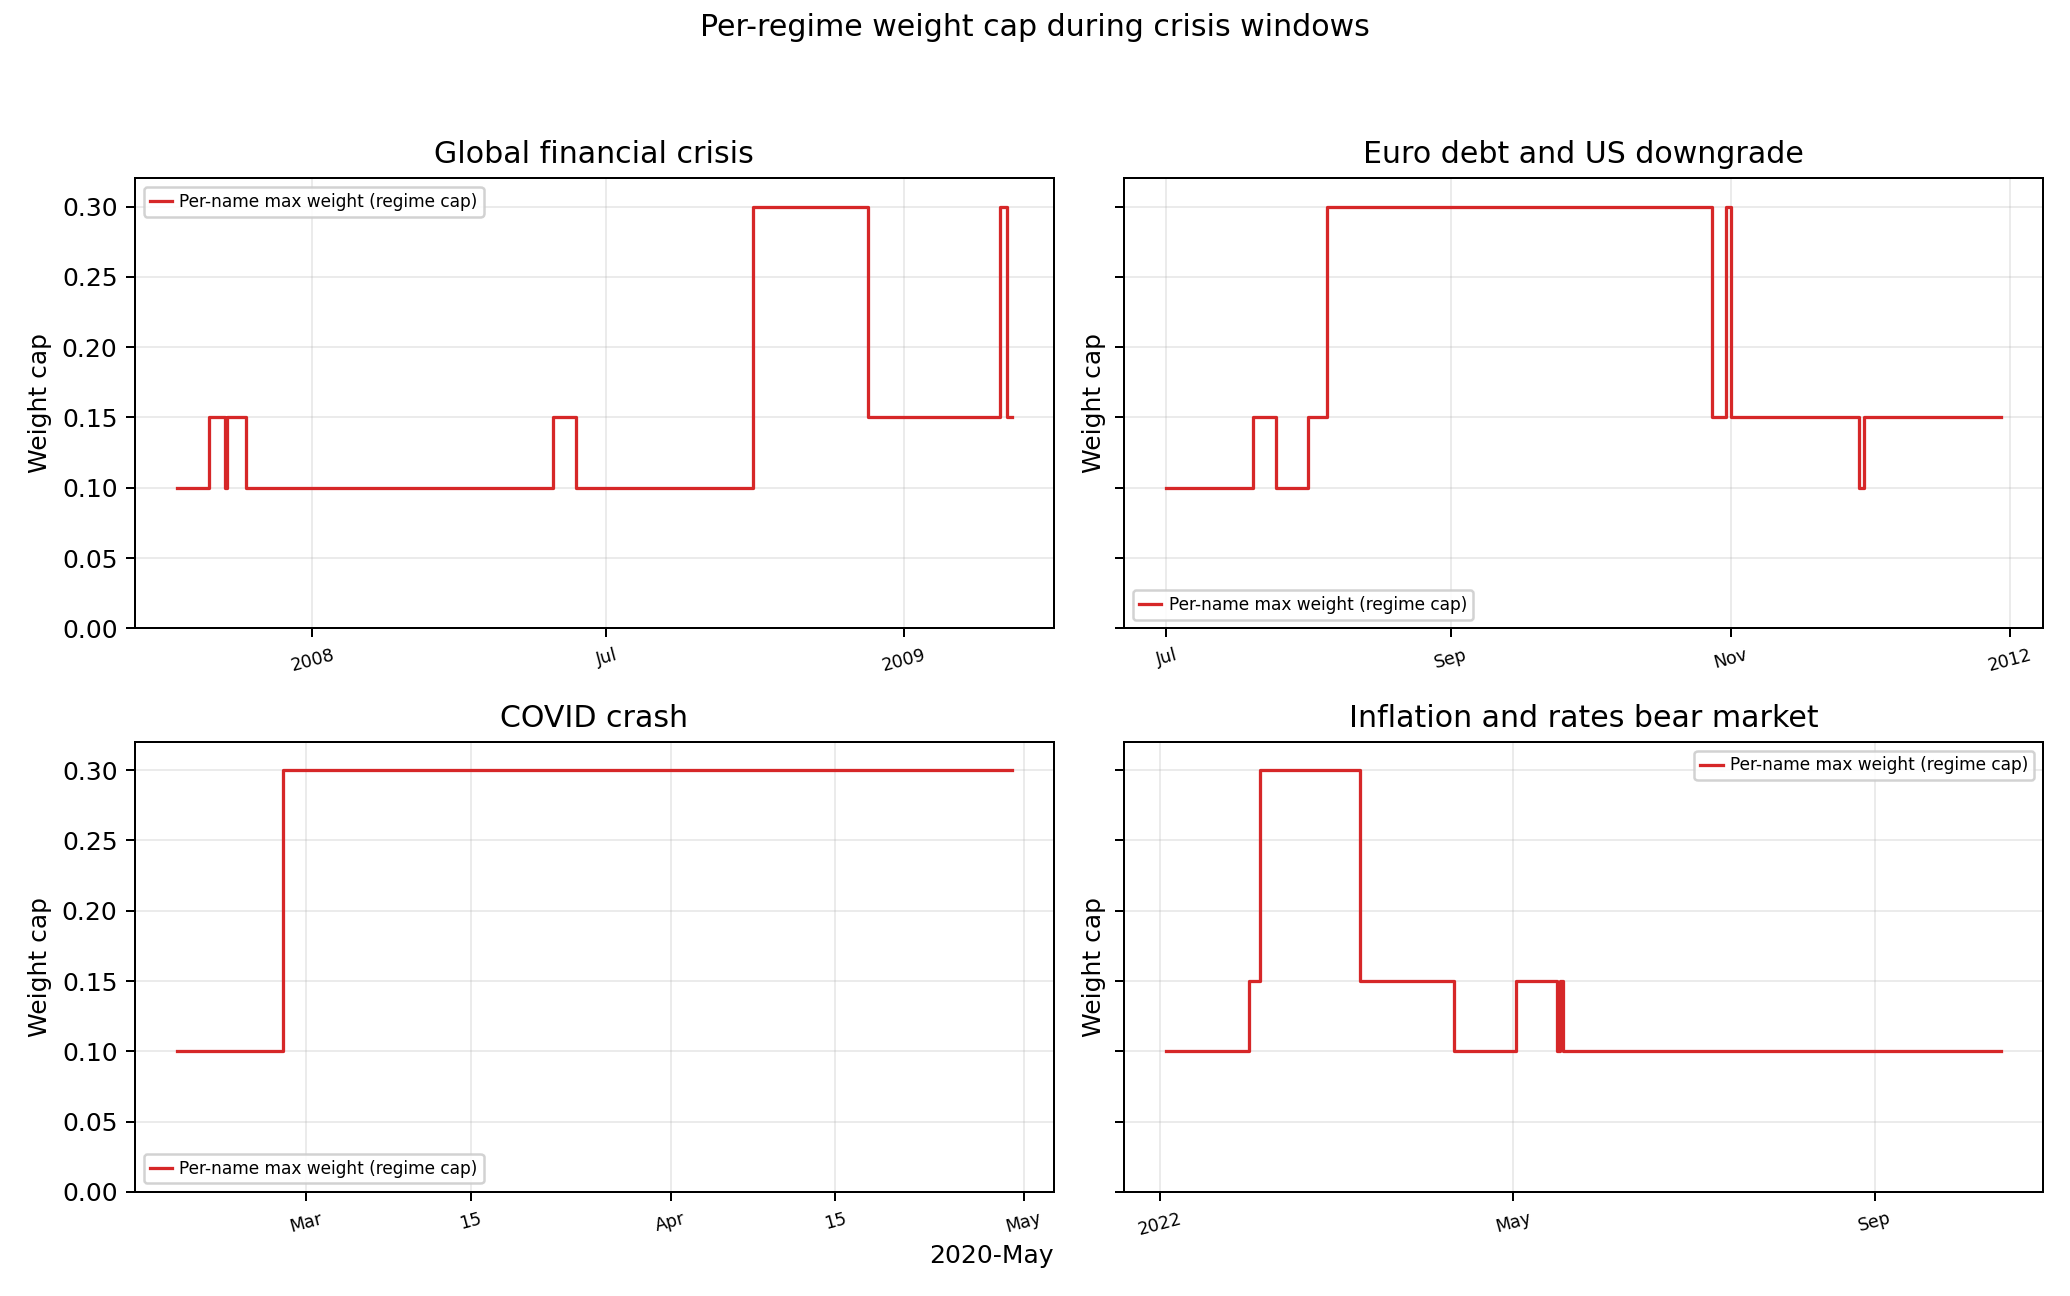
\includegraphics[width=0.96\linewidth]{crisis_bounds.png}
\caption{Per-regime maximum weight (the cap) during the same crisis windows --- the lever that switches gears: 30\% lets the portfolio concentrate (Bullish, ordered), 15\% is the balanced Neutral setting, and 10\% forces the diversified equal-weight book (Bearish, disordered). The minimum weight is zero throughout; in Bearish the cap is 10\%.}
\end{figure}

\begin{table}[H]
\centering
\begingroup
\scriptsize
\setlength{\tabcolsep}{3pt}
\resizebox{0.98\linewidth}{!}{\begin{tabular}{lrrrrr}
\hline
Crisis & Cum. return & Ann. vol & Sharpe & Max DD & Avg per-name cap \\
\hline
Global financial crisis & -46.78\% & 29.45\% & -1.23 & -47.42\% & 14.18\% \\
Euro debt and US downgrade & 2.00\% & 21.69\% & 0.18 & -11.86\% & 21.38\% \\
COVID crash & -6.06\% & 63.98\% & -0.42 & -26.86\% & 27.25\% \\
Inflation and rates bear market & -30.18\% & 32.81\% & -1.12 & -31.68\% & 13.26\% \\
\hline
\end{tabular}
}
\endgroup
\caption{Crisis-window performance and the average per-name regime cap for the entropy-regime strategy.}
\end{table}

\subsection{Market phases and transitions}

The market-phase classifier is intentionally simple, because the phase is just the strategy's gear selector along the ordered--disordered spectrum: Bullish (ordered) tells it to concentrate and speculate, Neutral keeps it balanced, and Bearish (disordered) tells it to diversify toward equal weight. It labels each day from the active-universe average entropy alone, comparing it to rolling, causal 33rd/67th percentile bands; the equal-weight top-10 proxy still supplies the rolling return, drawdown, and volatility that are reported per phase as descriptive diagnostics. The same phase labels set the per-name weight cap and color the cumulative-wealth chart.

\begin{figure}[H]
\centering
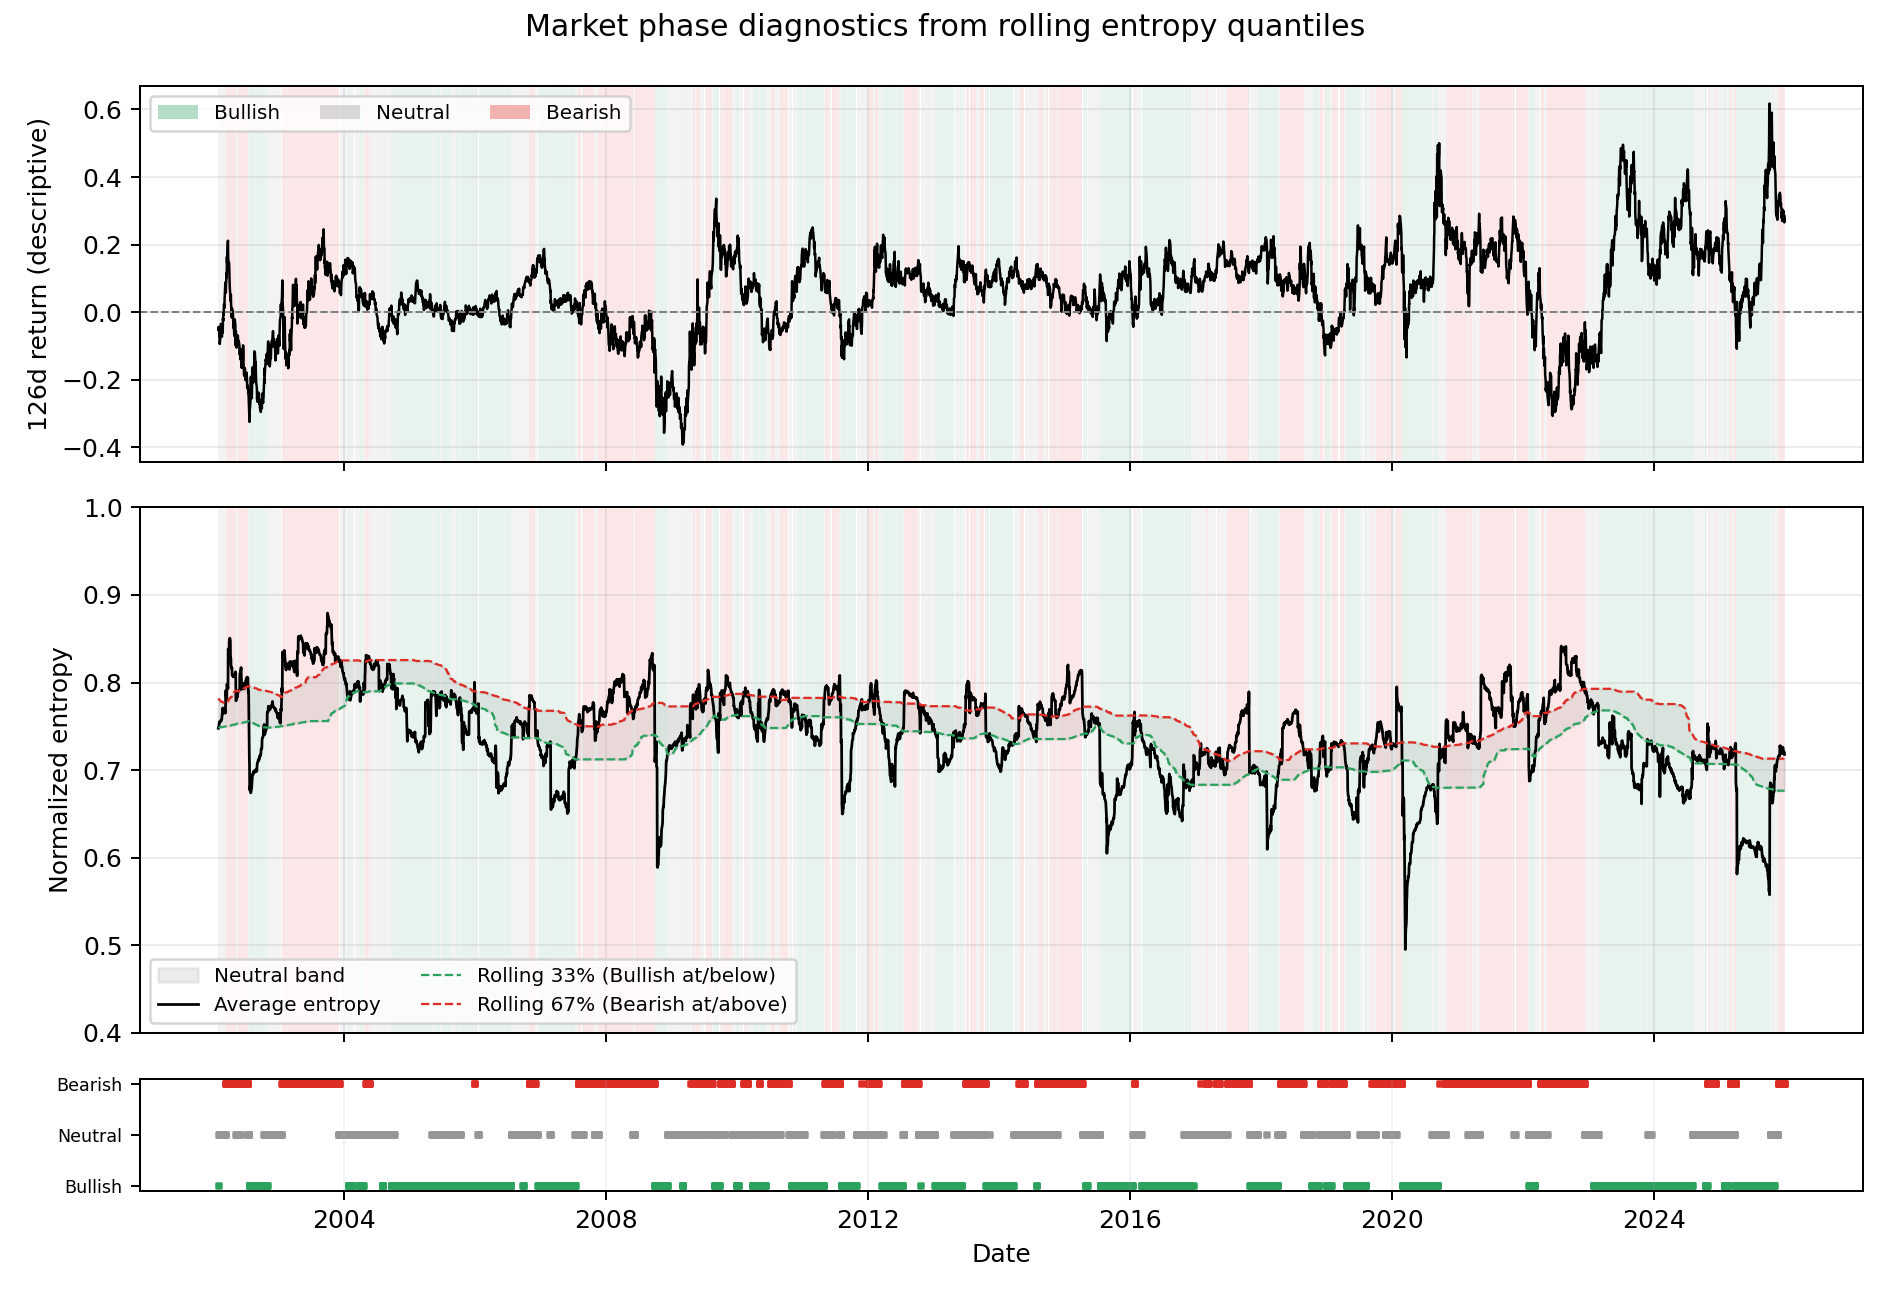
\includegraphics[width=0.96\linewidth]{market_phase_diagnostics.png}
\caption{Market-phase diagnostics: 126-day rolling return (descriptive), the average entropy with its rolling 33rd/67th percentile bands (vertical axis zoomed to 0.4--1.0, Neutral band shaded), and the daily Bullish/Neutral/Bearish label. The two bands split the entropy spectrum into the strategy's three gears --- below the 33rd percentile the market is ordered (concentrate), above the 67th it is disordered (diversify), and in between it is balanced.}
\end{figure}

% (standalone rolling-quantile figure removed: it duplicated the entropy panel above)

\begin{table}[H]
\centering
\begingroup
\scriptsize
\setlength{\tabcolsep}{3pt}
\resizebox{0.94\linewidth}{!}{\begin{tabular}{lrrrrrrr}
\hline
Phase & Days & Share & Ann. mean ret. & Mean 126d ret. & Mean entropy & Mean vol. & Mean drawdown \\
\hline
Bullish & 2371 & 39.42\% & 22.10\% & 8.11\% & 0.702 & 18.47\% & -4.44\% \\
Neutral & 1713 & 28.48\% & 8.60\% & 5.22\% & 0.750 & 18.96\% & -5.77\% \\
Bearish & 1931 & 32.10\% & 9.17\% & 4.78\% & 0.783 & 19.04\% & -5.78\% \\
\hline
\end{tabular}
}
\endgroup
\caption{Market-phase summary over the 2002--2025 evaluation period (6{,}015 optimized days).}
\end{table}

\begin{figure}[H]
\centering
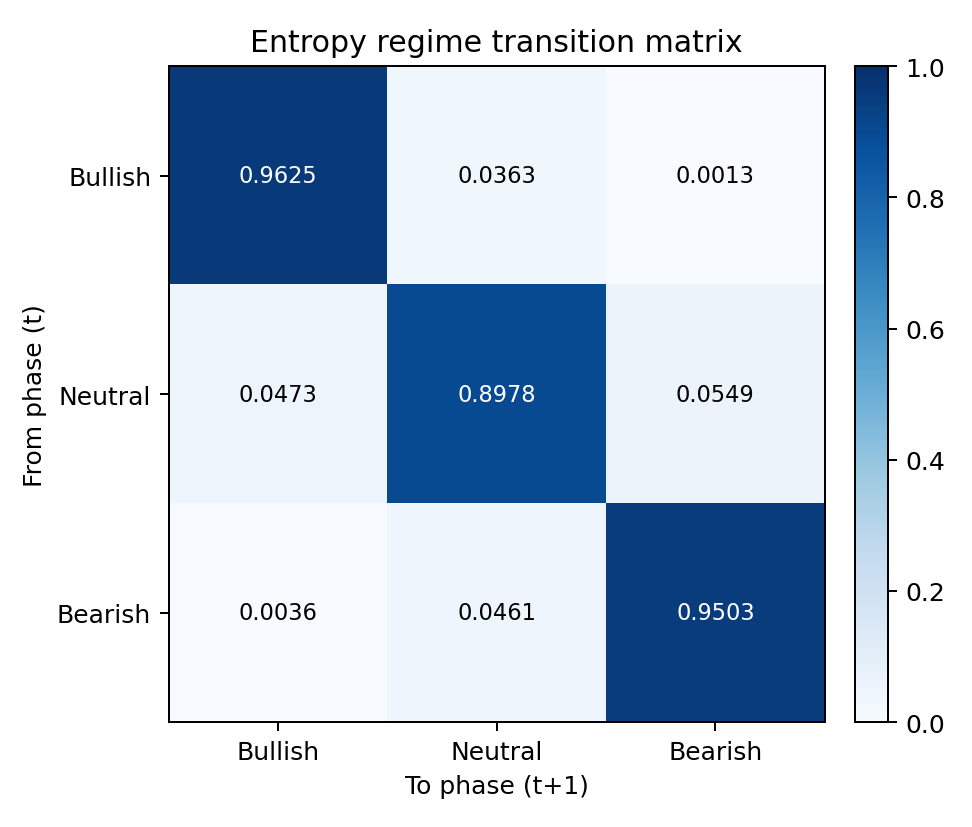
\includegraphics[width=0.66\linewidth]{market_phase_transition_heatmap.png}
\caption{Empirical transition matrix between the entropy regimes: each cell is the probability of moving from today's phase (row) to the next trading day's phase (column). The strong diagonal shows that the ordered, balanced, and disordered gears persist from day to day, which is what makes a regime-driven cap usable.}
\end{figure}

\subsection{Feasibility, traded names, and bound usage}

\begin{figure}[H]
\centering
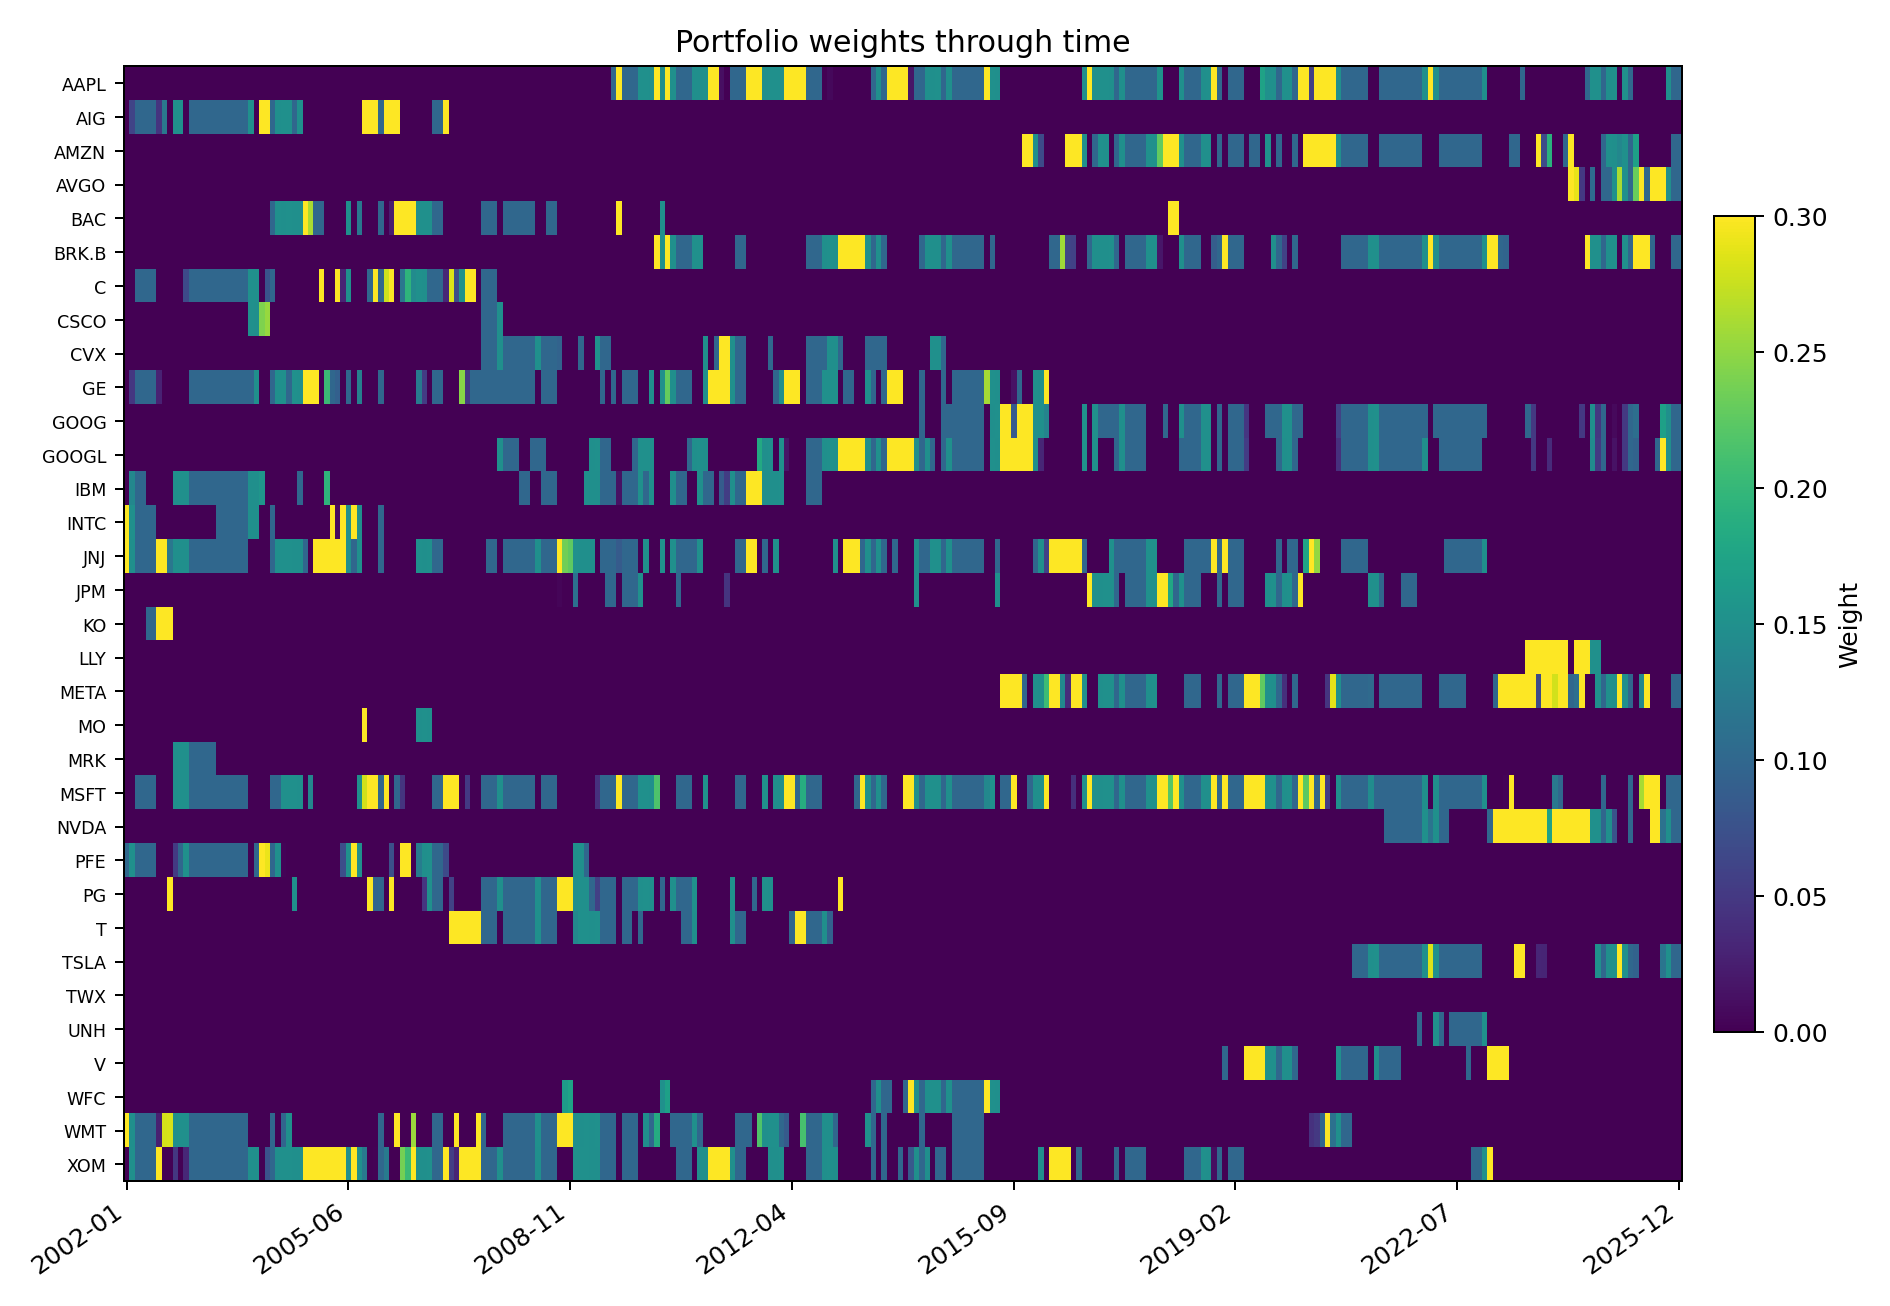
\includegraphics[width=0.96\linewidth]{weight_exposure_heatmap.png}
\caption{Portfolio weights. Inactive names are 0\%; active names are bounded below by 0 and above by the current entropy-regime cap (30\%/15\%/10\% for Bullish/Neutral/Bearish).}
\end{figure}

\begin{figure}[H]
\centering
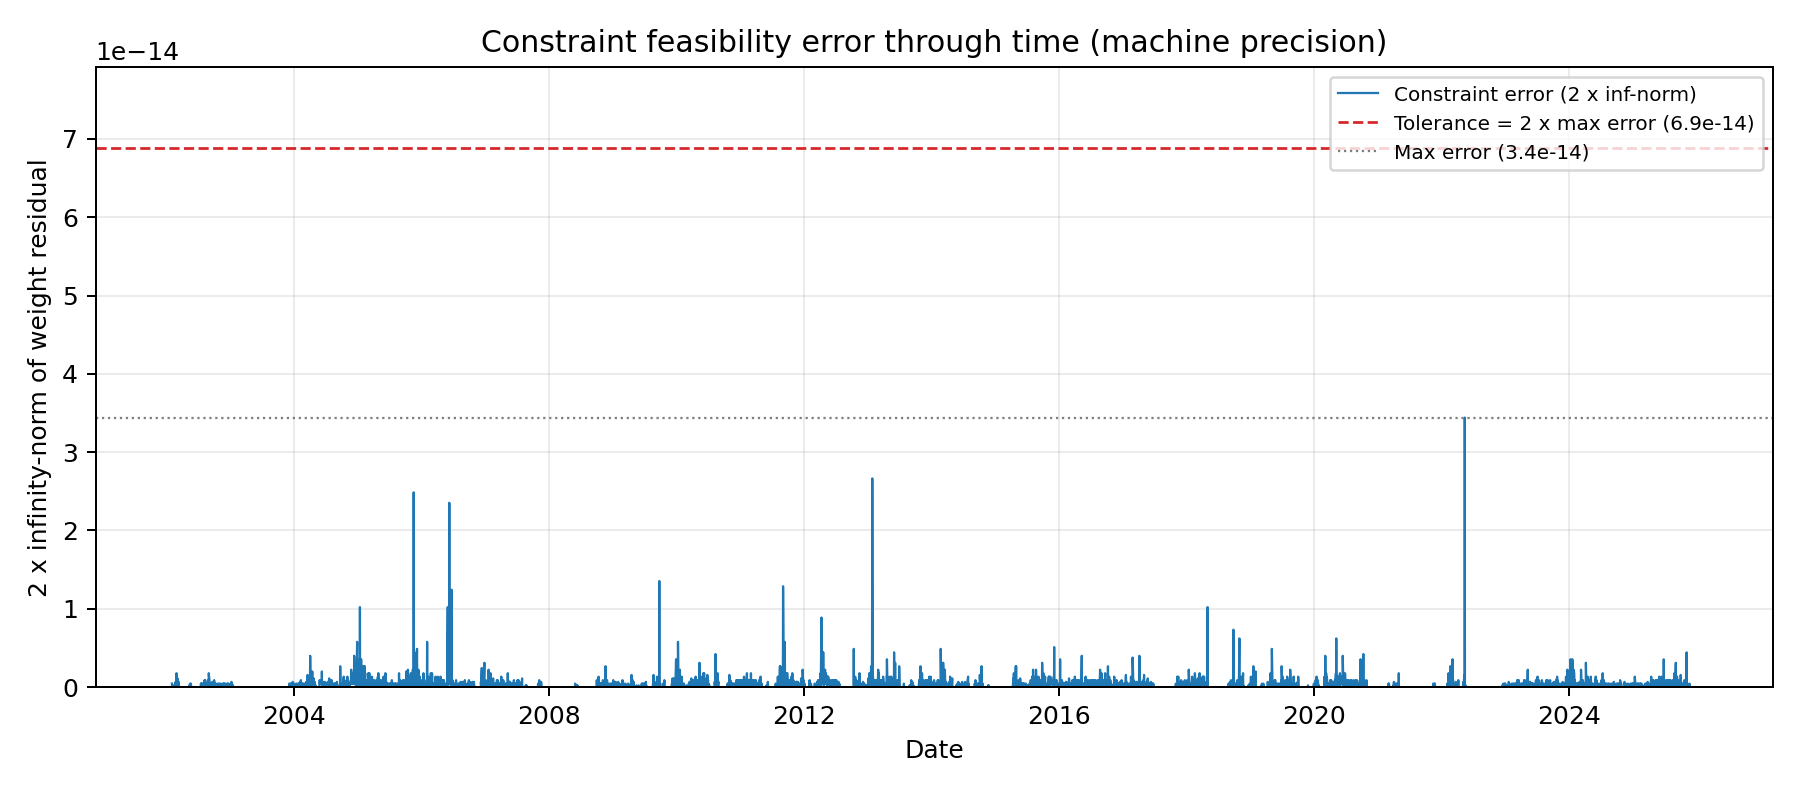
\includegraphics[width=0.96\linewidth]{weight_sum_error.png}
\caption{Constraint feasibility error through time: twice the infinity norm of the weight residual, against a tolerance drawn at double the worst observed error. The error never leaves machine precision (order $10^{-15}$), confirming that every daily solution is feasible.}
\end{figure}

\begin{figure}[H]
\centering
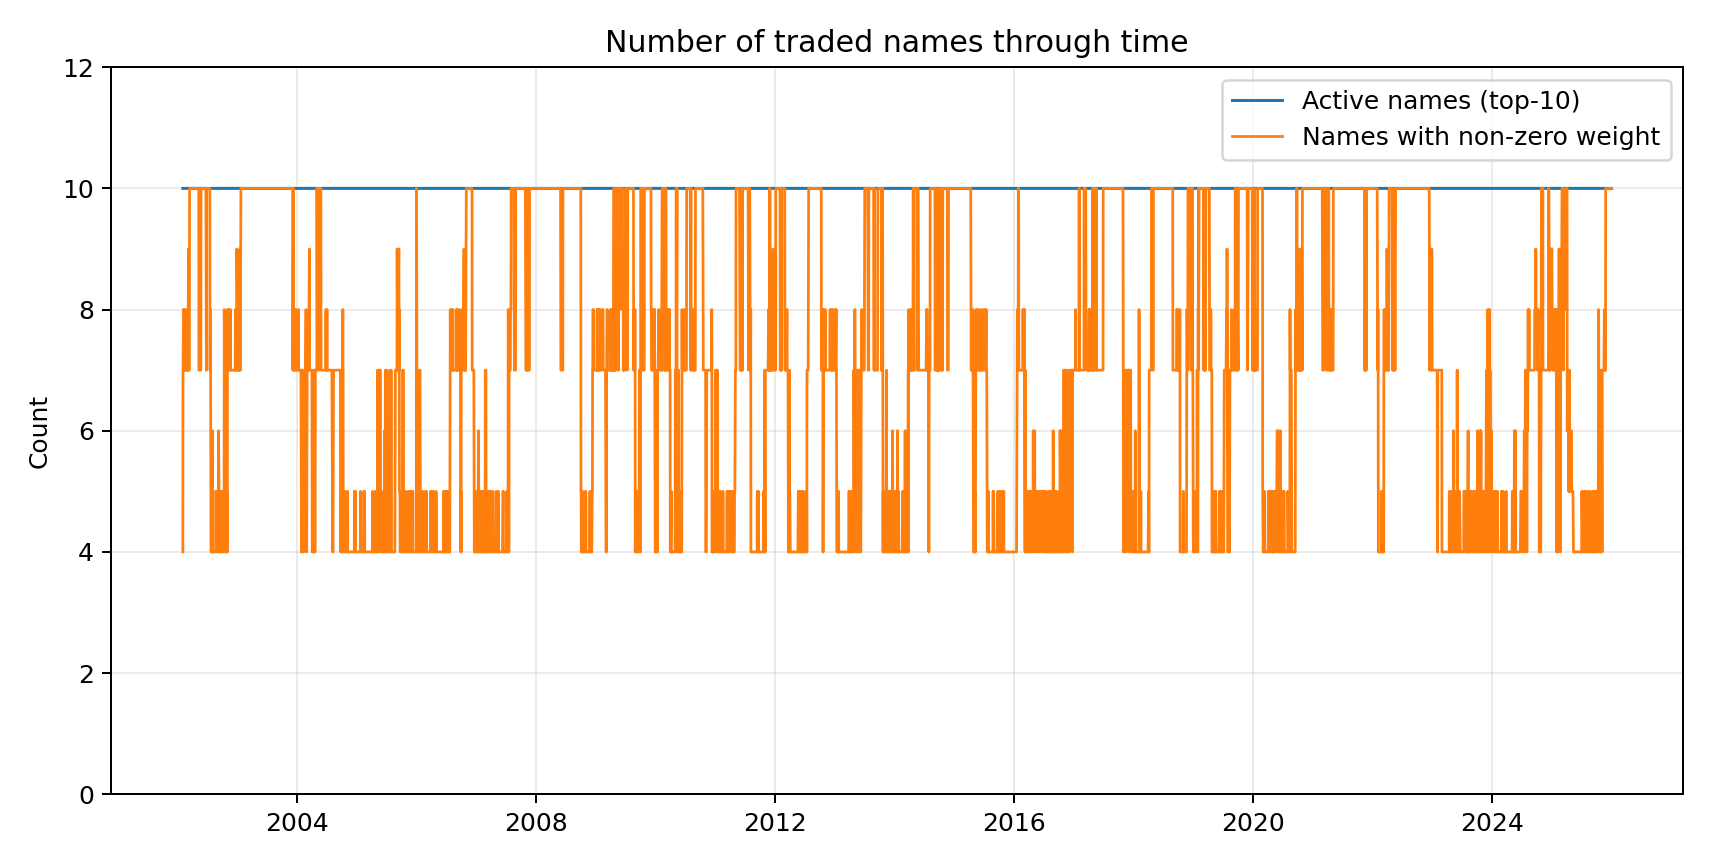
\includegraphics[width=0.86\linewidth]{traded_names_over_time.png}
\caption{Number of active and invested names through time.}
\end{figure}

\begin{figure}[H]
\centering
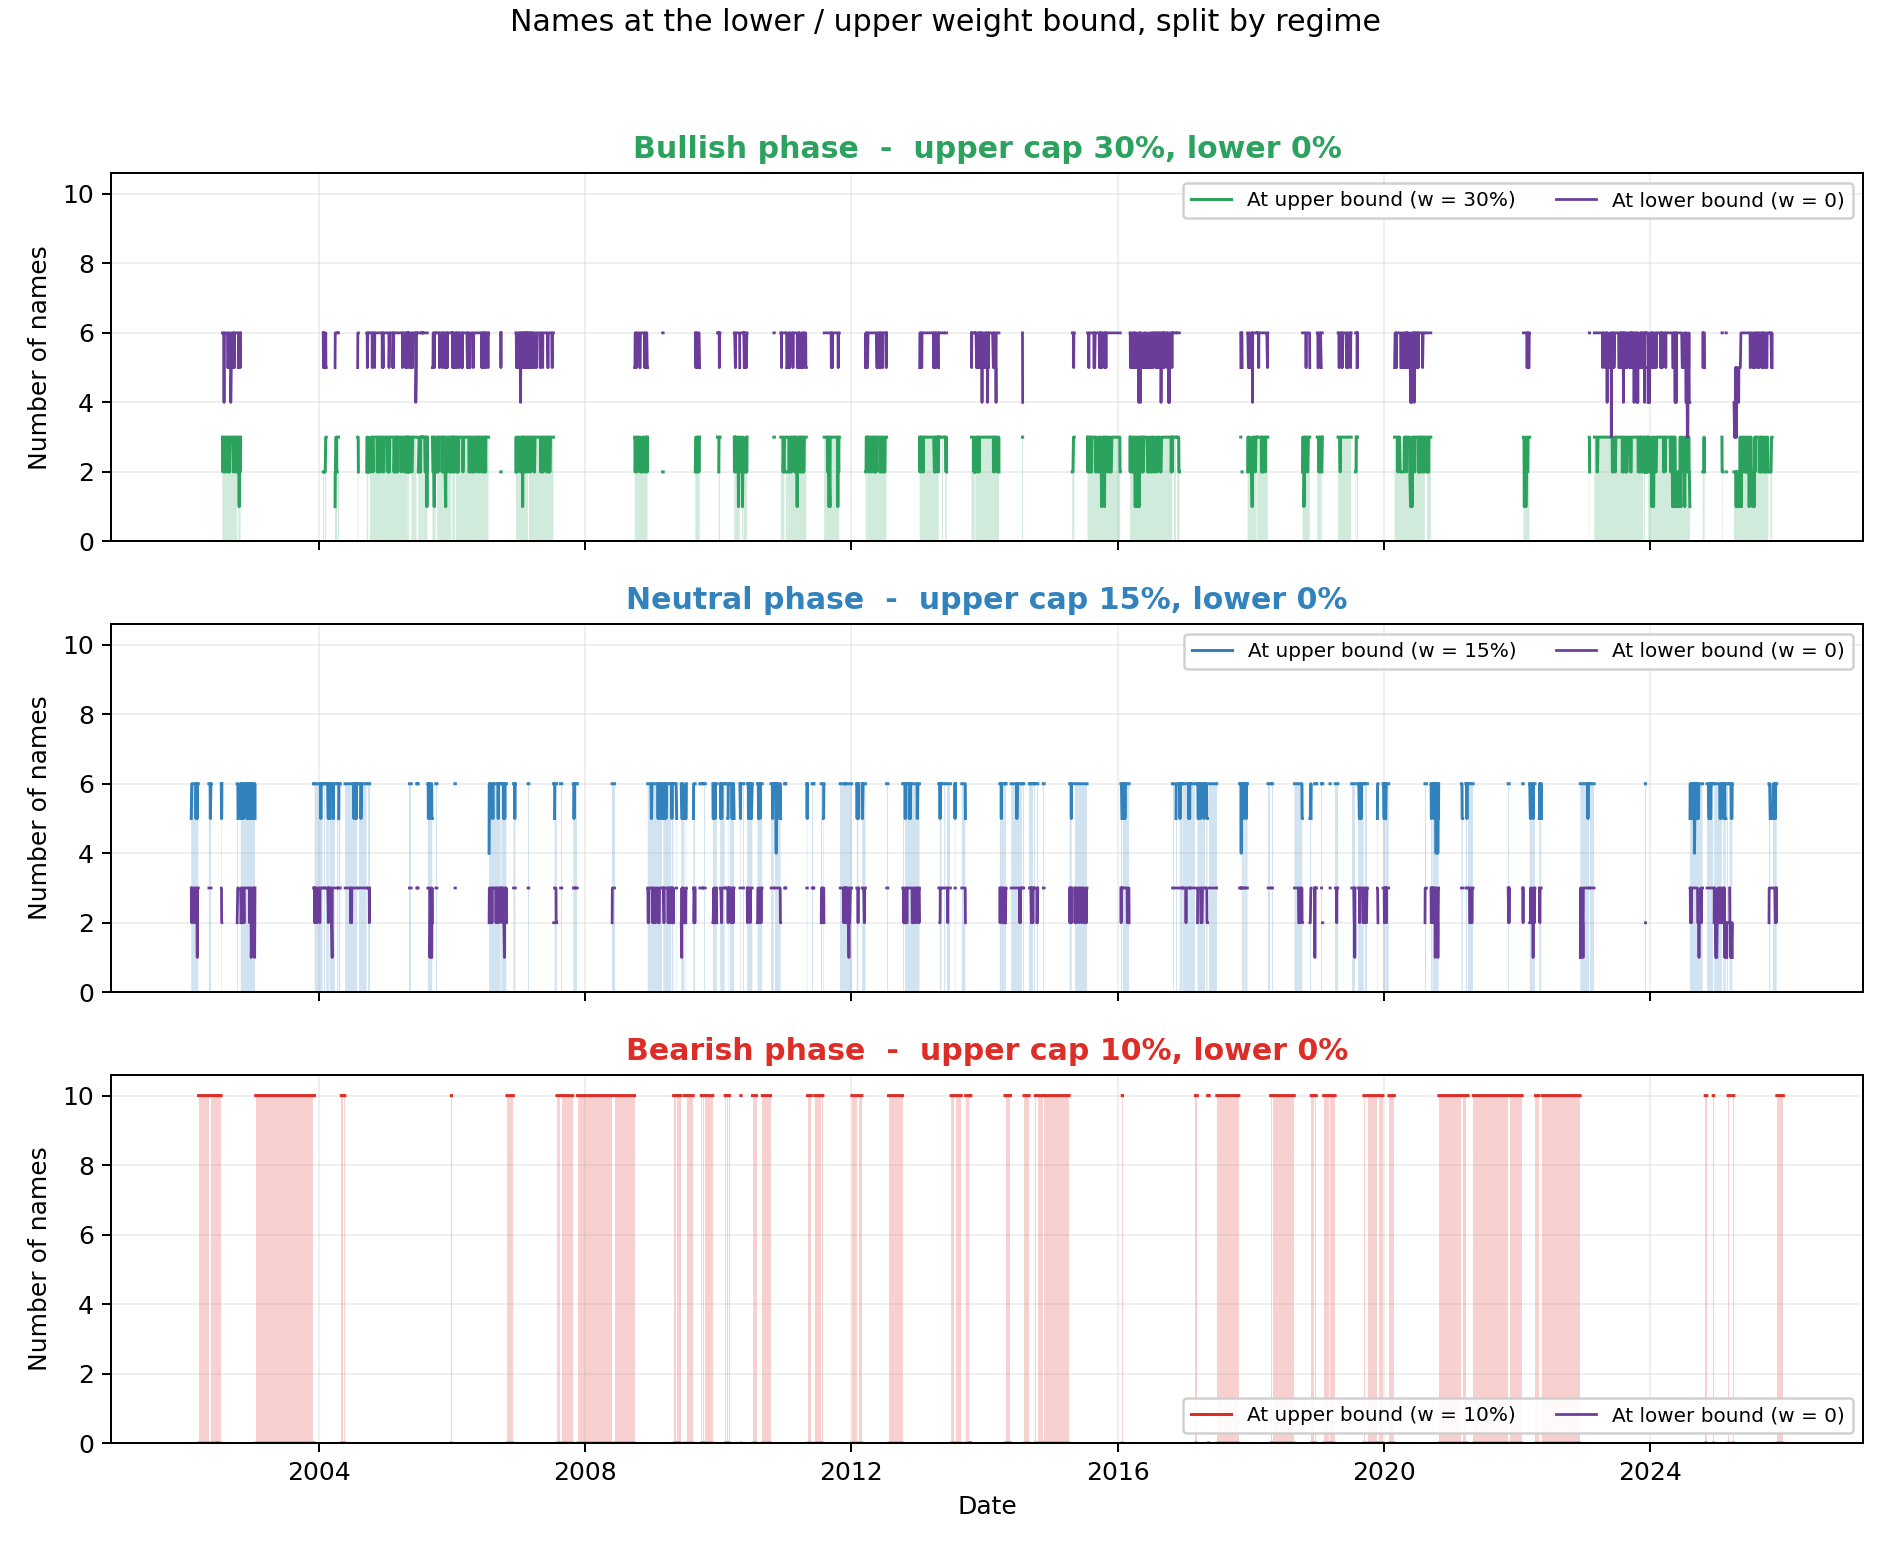
\includegraphics[width=0.86\linewidth]{bound_usage.png}
\caption{Number of names at the lower bound (weight 0) and at the upper bound (the regime cap), split into the three regimes --- a direct read of which gear is engaged. Concentration in the ordered Bullish gear pushes names against the 30\% cap; in the disordered Bearish gear every name sits at the 10\% cap (equal weight), so the upper-bound count equals the active count and the book is fully diversified.}
\end{figure}

\begin{figure}[H]
\centering
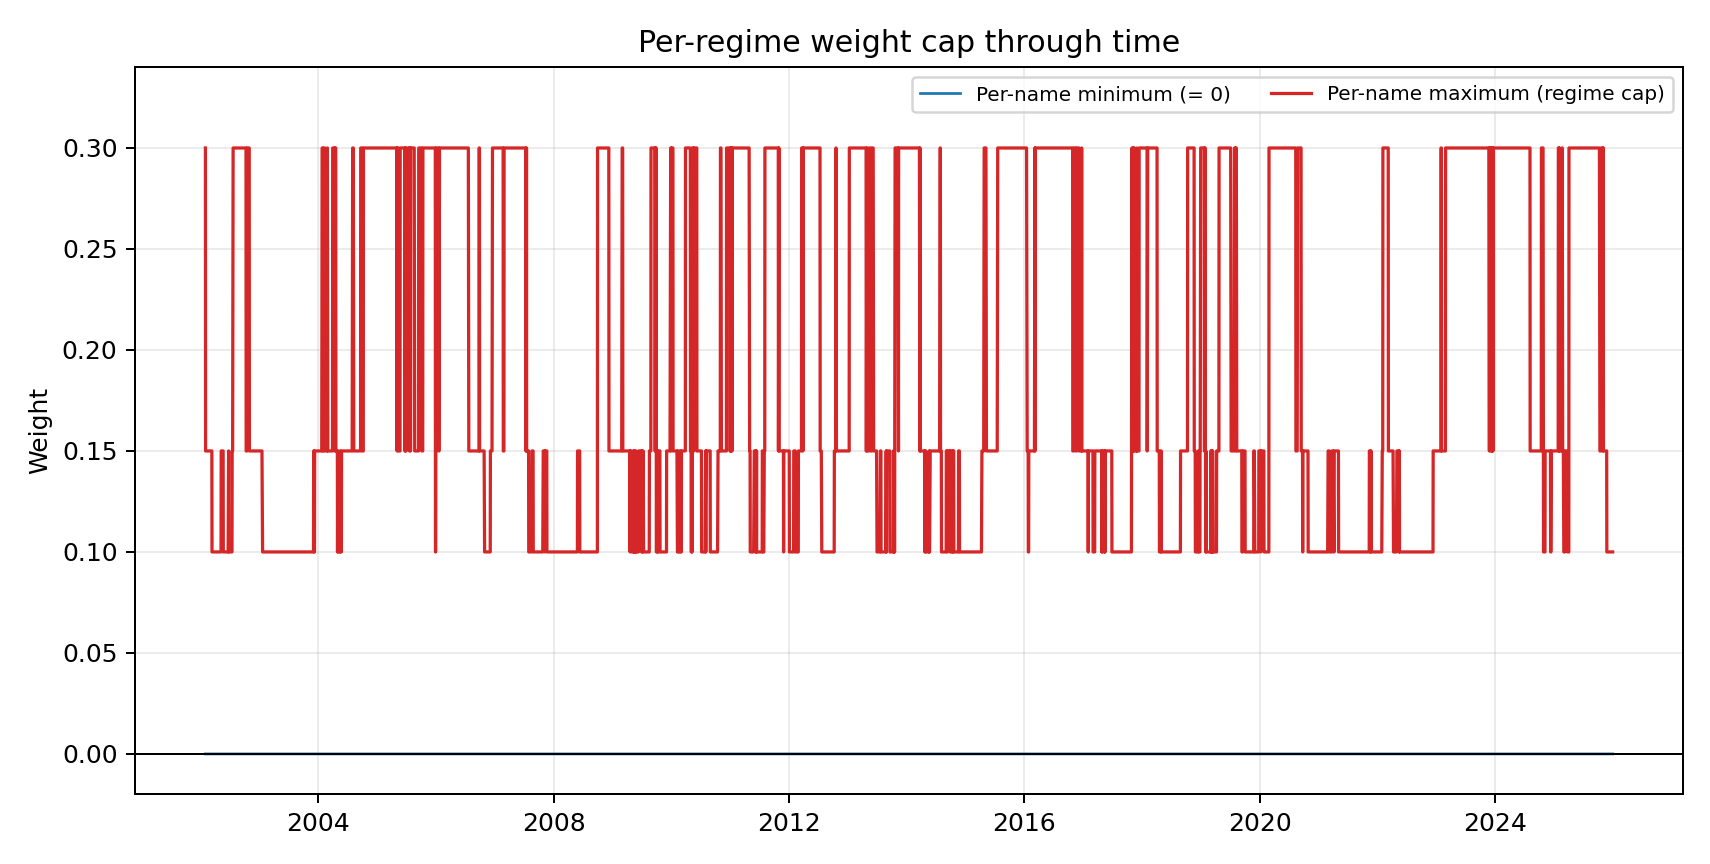
\includegraphics[width=0.86\linewidth]{dynamic_bounds_over_time.png}
\caption{Per-name maximum weight (the regime cap) through time; the minimum is flat at zero. The cap steps between 30\%, 15\%, and 10\% as the entropy regime changes --- the single lever that shifts the strategy between concentrating (ordered), balanced, and diversifying toward equal weight (disordered).}
\end{figure}

% (bound-usage table removed: no candidate-grid calibration in the simplified project)

\section{Conclusions}

This project set out to solve a practical problem --- building a daily long-only portfolio over a moving top-10 universe --- with a strategy that speculates when the market is ordered and diversifies when it is disordered. The mechanism that makes the strategy work is a single algorithm: a transparent, look-ahead-free rolling Shannon entropy that places the market on its ordered-to-disordered spectrum. Entropy is used \emph{only} as this regime filter; the expected-return input is the plain rolling mean. Around that one number the rest of the rule is intentionally minimal --- it uses adjusted price-index inputs, keeps inactive tickers at zero, restricts trading to the genuine top-10 by date, and sets the per-name weight cap directly from the entropy regime: a standard SLSQP mean-variance solve at a 30\% (Bullish) or 15\% (Neutral) cap, and an explicit equal-weight book in the disordered Bearish regime. Over the 2002--2025 sample the strategy improves annualized return, Sharpe ratio, and maximum drawdown relative to a naive max-Sharpe baseline, the equal-weight top-10, and the S\&P 500 total-return buy-and-hold, while maintaining feasible weights on every trading date. The entropy regime is therefore operational, not merely descriptive: the three labels are the three gears of the speculate-versus-diversify strategy.

The algorithm should be interpreted as a disciplined portfolio-construction method, not as a return forecaster. This is by design: the rolling mean is a deliberately weak tie-breaker, while the real decision --- \emph{how aggressively to act} --- is carried entirely by the entropy regime (the per-name cap and the speculate-versus-diversify switch). Entropy is kept directionless and scale-free precisely so that it measures market \emph{disorder} and nothing else, leaving direction to the rolling mean and risk to the covariance.

Potential improvements include adaptive binning, transaction-cost modeling, turnover constraints, and alternative entropy definitions such as permutation entropy~\cite{bandt}.

\addcontentsline{toc}{section}{References}
\begin{thebibliography}{9}
\bibitem{shannon}
C. E. Shannon, ``A Mathematical Theory of Communication,'' \textit{Bell System Technical Journal}, 1948.

\bibitem{markowitz}
H. Markowitz, ``Portfolio Selection,'' \textit{The Journal of Finance}, 1952.

\bibitem{philippatos}
G. C. Philippatos and C. J. Wilson, ``Entropy, Market Risk, and the Selection of Efficient Portfolios,'' \textit{Applied Economics}, 1972.

\bibitem{zhou}
R. Zhou, R. Cai, and G. Tong, ``Applications of Entropy in Finance: A Review,'' \textit{Entropy}, 2013.

\bibitem{hamilton}
J. D. Hamilton, ``A New Approach to the Economic Analysis of Nonstationary Time Series and the Business Cycle,'' \textit{Econometrica}, 1989.

\bibitem{jagannathan}
R. Jagannathan and T. Ma, ``Risk Reduction in Large Portfolios: Why Imposing the Wrong Constraints Helps,'' \textit{The Journal of Finance}, 2003.

\bibitem{bandt}
C. Bandt and B. Pompe, ``Permutation Entropy: A Natural Complexity Measure for Time Series,'' \textit{Physical Review Letters}, 2002.

\bibitem{nocedal}
J. Nocedal and S. Wright, \textit{Numerical Optimization}, Springer, 2006.

\bibitem{yfinance}
Yahoo Finance data accessed through the \texttt{yfinance} Python package. Adjusted closes are used with \texttt{auto\_adjust=True}.
\end{thebibliography}

\end{document}
